% !TEX program = xelatex
\documentclass{article}

\title{Notite examen - Sisteme de Operare}
\date{}
\author{Dinu Florin-Silviu \\ grupa 231}

\newcommand{\prim}{^\ensuremath{\prime}}
\newcommand{\secund}{^{\ensuremath{\prime\prime}}}

% \makeatletter
% \renewcommand{\@seccntformat}[1]{}
% \makeatother

\newenvironment{textColor}[1]{%
    \leavevmode\color{#1}\ignorespaces%
}{%
}%


\usepackage{tikz}
\usepackage{forest}
\usepackage{hyperref}
\usepackage{amsthm}
\usepackage{amssymb}
\usepackage[english]{babel}
\usepackage[a4paper, margin=3cm]{geometry}
\usepackage{enumitem}
\usepackage{listings}
\usepackage{fontspec}
\usepackage{xcolor}
\usepackage{textcomp}
\usepackage{graphicx}
\usepackage{tabularx}
\usepackage{pgfgantt}

\graphicspath{ {./img/} }

\newfontfamily{\ttconsolas}{Consolas}
\lstset{
%  tabsize=4,
extendedchars=true,
        basicstyle=\ttconsolas,
        % %upquote=false,
        % aboveskip=\baselineskip,
        columns=fixed,
        showstringspaces=false,
        extendedchars=true,
        breaklines=true,
        % prebreak = \raisebox{0ex}[0ex][0ex]{\ensuremath{\hookleftarrow}},
        showtabs=false,
        showspaces=false,
        identifierstyle=\ttfamily,
        % keywordstyle=\color[rgb]{0,0,1},
        % commentstyle=\color[rgb]{0.133,0.545,0.133},
        % stringstyle=\color[rgb]{0.627,0.126,0.941},
        % language=SQL
        frame=lines,
        literate=%
    {€}{\euro}1%
    {§}{\S}1%
    {°}{\textdegree{}}1%
    {ä}{{\"a}}1%
    {ö}{{\"o}}1%
    {ü}{{\"u}}1%
    {ß}{{\ss}}1%
    {Ä}{{\"A}}1%
    {Ö}{{\"O}}1%
    {Ü}{{\"U}}1%
    {µ}{\textmu}1%
    {¹}{{\textsuperscript{1}}}1%
    {²}{{\textsuperscript{2}}}1%
    {³}{{\textsuperscript{3}}}1%
    {¼}{\textonequarter}1%
    {½}{\textonehalf}1%
    {¢}{\textcent}1%
}


\tikzstyle{red state}=[
        draw = red,
        thick,
        fill = white,
        minimum size = 4mm,
        circle
    ]

\tikzstyle{blue state}=[
    draw = blue,
    thick,
    fill = white,
    minimum size = 4mm,
    circle
]

\tikzstyle{green state}=[
    draw = green,
    thick,
    fill = white,
    minimum size = 4mm,
    circle
]

\tikzset{
  gray box/.style={
    fill=gray!20,
    draw=gray,
    minimum width={1.5*#1ex},
    minimum height={2em},
  },
  annotation/.style={
    anchor=north,
  }
}

\newtheorem*{theorem}{Teorema}
\renewcommand\qedsymbol{QED}

\begin{document}
\pagenumbering{gobble}
\maketitle
\tableofcontents

\newpage
\pagenumbering{arabic}

\section[Ch3 Processes]{Processes}
\subsection*{States}
\begin{enumerate}
    \item New - e creat
    \item Running - se executa instructiunile
    \item Waiting - asteapta un eveniment
    \item Ready - asteapta sa fie asignat unui procesor
    \item Terminated - a terminat executia
\end{enumerate}

\begin{center}
    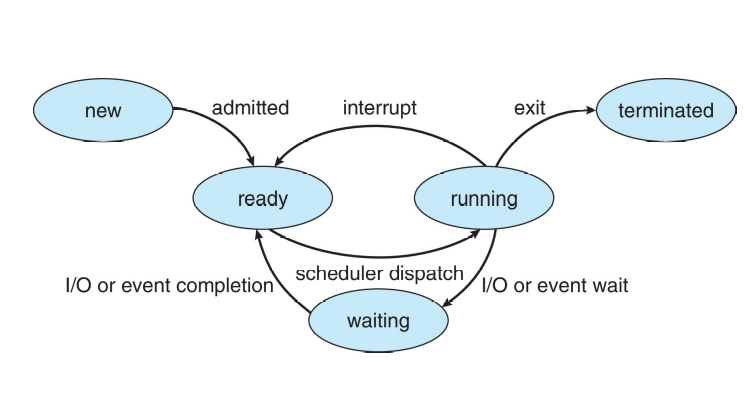
\includegraphics[scale=0.4]{1_procese.png}
\end{center}

\subsection*{Task control block}
\begin{enumerate}
    \item Process state
    \item Program counter (location of next instruction)
    \item CPU registers (contents of all process-centric registers)
    \item CPU scheduling information (priorities, scheduling queue pointers)
    \item Memory-management information (memory allocated to the process)
    \item Accounting information (CPU used, clock time since start, time limits)
    \item I/O status information (I/O devices allocated to the process, list of open files)
\end{enumerate}

\begin{center}
    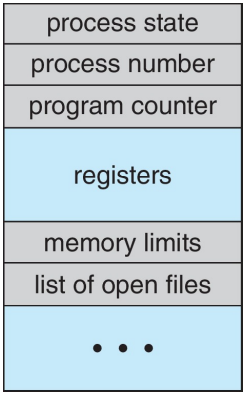
\includegraphics[scale=0.3]{2_taskcontrolblock.png}
\end{center}

\subsection*{Process scheduling}
\paragraph*{Process scheduler} selects among available processes for next execution on CPU core
\subparagraph*{Goal} - maximize CPU use, quickly switch processes onto CPU core
\subparagraph*{Scheduling queues} Ready queue and wait queue

\begin{center}
    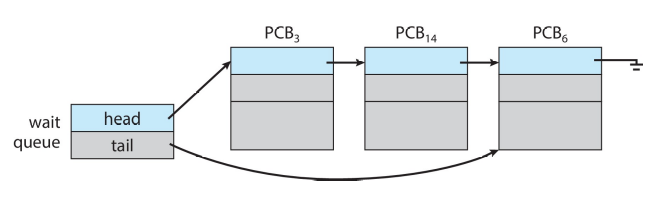
\includegraphics[scale=0.3]{3_processqueue.png}
\end{center}

\begin{center}
    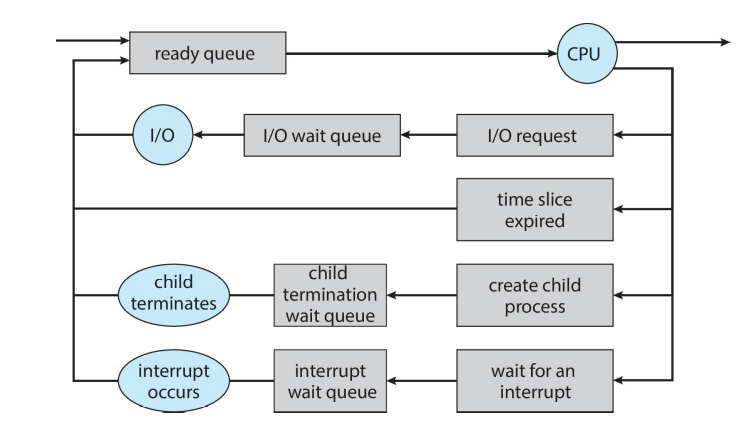
\includegraphics[scale=0.3]{4_indepthprocsched.png}
\end{center}

\subsection*{Context switch} When CPU switches to another process, the system must save the state of the old process and load the save state for the new process via a context switch
\paragraph*{Contextul} unui proces este reprezentat in PCB

\subsection*{Process creation}
\paragraph*{Parintii} creaza copii care, la randul lor, pot crea alte procese, formand un arbore de procese
\subparagraph*{PID} - process identifier ID
\paragraph*{Partajarea de resurse - optiuni}
\begin{enumerate}
    \item Parintii si copiii partajeaza toate resursele
    \item Copiii folosesc o submultime a resurselor parintilor
    \item Parintii si copiii nu partajeaza nicio resursa
\end{enumerate}
\paragraph*{Executie - optiuni}
\begin{enumerate}
    \item Parintii si copiii se executa concurent
    \item Parintele asteapta sa termine copilul
\end{enumerate}

\paragraph*{Spatiu de adresa}
\begin{enumerate}
    \item Copilul e un duplicat al parintelui
    \item Copilul are un program incarcat in el
\end{enumerate}

\paragraph*{Exemple UNIX}
\begin{enumerate}
    \item fork() - syscall pentru crearea de noi procese
    \item exec() - syscall dupa fork() ca sa inlocuiasca memory space-ul cu un alt program
    \item wait() - parintele asteapta sa termine copilul
\end{enumerate}

\subsection*{Process termination}
\paragraph*{exit()} - procesele executa ca ultima instructiune syscallul exit() care returneaza statusul catre parinte via wait() si resursele sunt dealocate de sistem
\paragraph*{abort()} - parintele poate termina oricand copilul. Unele din motive sunt: copilul a depasit resursele alocate, ceea ce i s-a cerut copilului nu mai este necesar, parintele a apelat exit() si sistemul nu mai lasa copilul sa continue in acest caz (terminarea in cascada)
\paragraph*{Zombie} nu mai are parinte care sa astepte (nu s-a invocat wait())
\begin{center}
    \begin{lstlisting}
pid_t pid = fork();
if(pid)
        sleep(5);
else
        exit(0);
return 0;
    \end{lstlisting}
\end{center}
\paragraph*{Orfan} parintele s-a terminat fara sa invoce wait()

\begin{center}
    \begin{lstlisting}
pid_t pid = fork();
if(pid)
        exit(0);
else{
    sleep(5);
}

return 0;
    \end{lstlisting}
\end{center}

\subsection*{Interprocess Communication}
\paragraph*{Procesele} pot fi independente sau sa coopereze
\subparagraph*{Cooperarea} inseamna ca procesul poate fi afectate sau afecta alte procese, inclusiv datele partajate
\paragraph*{Motive pentru cooperare}
\begin{enumerate}
    \item Partajarea de informatie
    \item Viteza de calcul mai mare
    \item Modularitate
    \item Convenienta
\end{enumerate}
\paragraph*{IPC - 2 modele}
\begin{enumerate}
    \item memorie partajata
    \item pasare de mesaje
\end{enumerate}

\begin{center}
    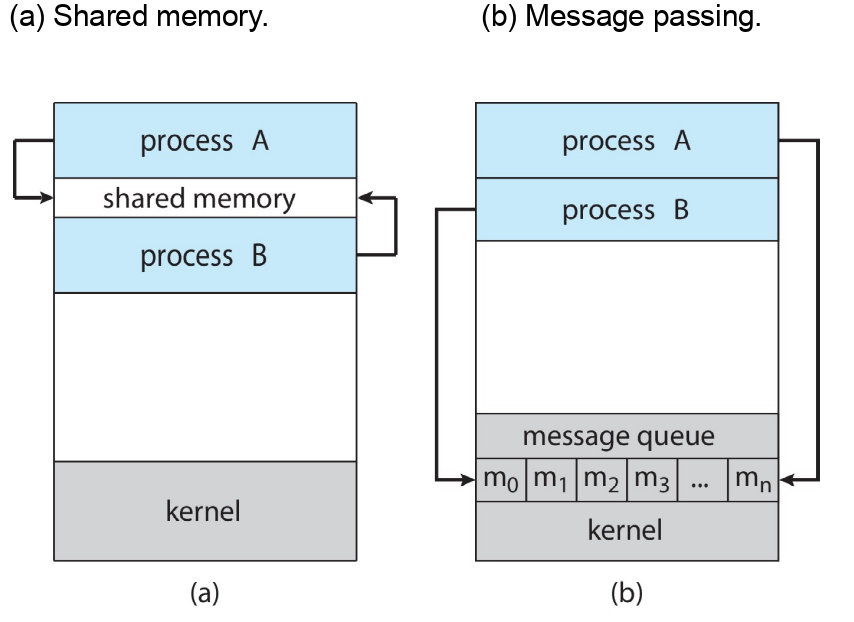
\includegraphics[scale=0.3]{5_ipc.png}
\end{center}

\subsection*{Shared memory}

\begin{center}
    \begin{lstlisting}
#include <stdio.h>
#include <unistd.h>
#include <stdlib.h>
#include <sys/wait.h>
#include <sys/mman.h>
#include <fcntl.h>

int collatz(int32_t *shmColl, int32_t n, int32_t i){
    shmColl[i] = n;
    if(n == 1)
        return i + 1;
    
    if(n % 2)
        n = 3 * n + 1;
    else
        n /= 2;

        return collatz(shmColl, n, ++i);
}

int main(int argc, char **argv){
    if(argc<2){
        printf("Prea putine argumente\n");
        return -1;
    }

    printf("Starting parent %d\n", getpid());

    pid_t pids[argc];

    char *shmName = "lab5collatz";
    int64_t shmFd = shm_open(shmName, O_CREAT | O_RDWR, S_IRUSR | S_IWUSR);
    if(shmFd < 0){
        printf("Can't open shared memory\n");
        return -2;
    }

    size_t shmSize = getpagesize() * argc;

    int64_t ftruncateReturn = ftruncate(shmFd, shmSize);
    if(ftruncateReturn == -1){
        printf("Can't truncate\n");
        shm_unlink(shmName);
        return -3;
    }

    for(int64_t i = 0; i < argc; ++i){
        pids[i] = fork();
        if(pids[i] < 0){
            return -4;
        } 

        if(pids[i] == 0) {
            int32_t *shmColl = mmap(NULL, getpagesize(), PROT_WRITE | PROT_READ, MAP_SHARED, shmFd, getpagesize() * i);
            if (shmColl == MAP_FAILED) {
                printf("Map failed\n");
                shm_unlink(shmName);
                return -5;
            }

            int32_t x = atoi(argv[i + 1]);
            int32_t shmSize = collatz(shmColl, x, 0);
            printf("%d: ", x);
            for (int32_t j = 0; j < shmSize; ++j)
                printf("%d ", shmColl[j]);

            printf("\n");
            return 0;
        }
    }

    for(int32_t i = 0; i < argc; ++i){
        printf("Done parent %d Me %d\n", getppid(), getpid());
        wait(NULL);
    }

    shm_unlink(shmName);
    munmap(0, getpagesize() * argc);

    return 0;
}
    \end{lstlisting}
\end{center}

\paragraph*{Producer-consumer}: producatorul produce informatie care e consumata de consumator
\subparagraph*{2 variante}
\begin{enumerate}
    \item unbounded-buffer - nu are limite practice asupra marimii bufferului
          \begin{enumerate}
              \item producatorul nu asteapta
              \item consumatorul asteapta daca nu e buffer de consumat
          \end{enumerate}
    \item bounded-buffer - toate bufferele au marime fixa
          \begin{enumerate}
              \item producatorul trebuie sa astepte daca toate bufferele sunt full
              \item consumatorul asteapta daca nu e buffer pe care sa-l consume
          \end{enumerate}
\end{enumerate}

\paragraph*{Umplerea TUTUROR bufferelor} se face cu un counter care e 0, e incrementat de producator cu fiecare buffer si decrementat de consumator dupa ce il consuma

\paragraph*{Race condition}

\begin{center}
    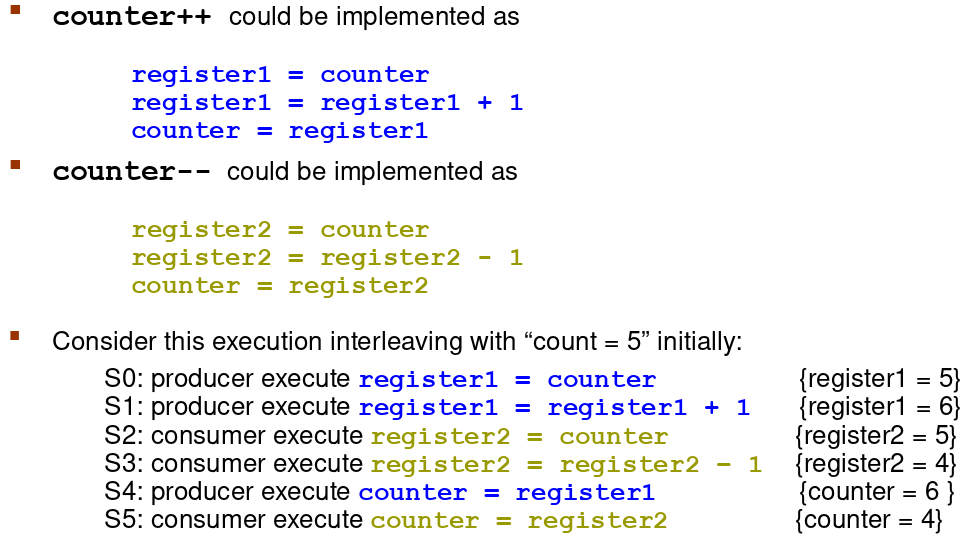
\includegraphics[scale=0.3]{6_racecondition.png}
\end{center}


\subsection*{Message passing}
\paragraph*{2 operatii}: send(message), receive(message)
\paragraph*{Communication link}
\begin{enumerate}
    \item Physical
          \begin{enumerate}
              \item Shared memory
              \item Hardware bus
              \item Network
          \end{enumerate}
    \item Logical
          \begin{enumerate}
              \item Direct sau indirect
              \item Sincron sau asincron
              \item Buffering automat sau explicit
          \end{enumerate}
\end{enumerate}

\paragraph*{Comunicarea directa}
\subparagraph*{Se denumesc explicit} send(P, msg) sau receive(Q, msg)
\subparagraph*{Avantaje}
\begin{enumerate}
    \item Linkurile sunt stabilite automat
    \item Linkurile sunt asociate cu exact o pereche de procese care comunica
    \item Intre 2 procese este exact 1 link
    \item Linkul poate fi unidrectional, dar de obicei, e bidirectional
\end{enumerate}

\paragraph*{Comunicarea indirecta}
\subparagraph*{Mesajele vin din mailboxes (ports)} Fiecare mailbox are ID unic, procesele pot comunica doar daca partajeaza un mailbox
\subparagraph*{Proprietatile linkului de comunicare}
\begin{enumerate}
    \item Linkurile sunt stabilite doar daca e un mailbox comun
    \item Un link poate fi asociat cu mai multe procese
    \item Perechile de procese pot avea in comun mai multe linkuri
    \item Linkul poate fi unidirectional sau bidirectional
\end{enumerate}
\subparagraph*{Operatii}
\begin{enumerate}
    \item Crearea de mailbox (port)
    \item Send and receive
    \item Delete
\end{enumerate}
\subparagraph*{Primitive} send(A, msg), receive(A, msg)

\paragraph*{Pasarea de mesaje}
\begin{enumerate}
    \item Blocking
          \begin{enumerate}
              \item Blocking send
              \item Blocking receive
          \end{enumerate}
    \item Non-blocking
          \begin{enumerate}
              \item Non-blocking send
              \item Non-blocking receive
          \end{enumerate}
    \item Alte combinatii: daca avem send si receive blocking, avem \textbf{rendezvous}
\end{enumerate}

\paragraph*{Buffering}
\subparagraph*{Queue} atasata unui link
\subparagraph*{3 implementari:}
\begin{enumerate}
    \item Zero capcity - fara mesaje pe link. Senderul asteapta pentru receiver (rendezvous)
    \item Bounded capacity - lungime finita de n mesaje. Senderul asteapta daca linkul e full
    \item Unbounded capacity - lungime infinita. Senderul nu asteapta niciodata
\end{enumerate}

\begin{center}
    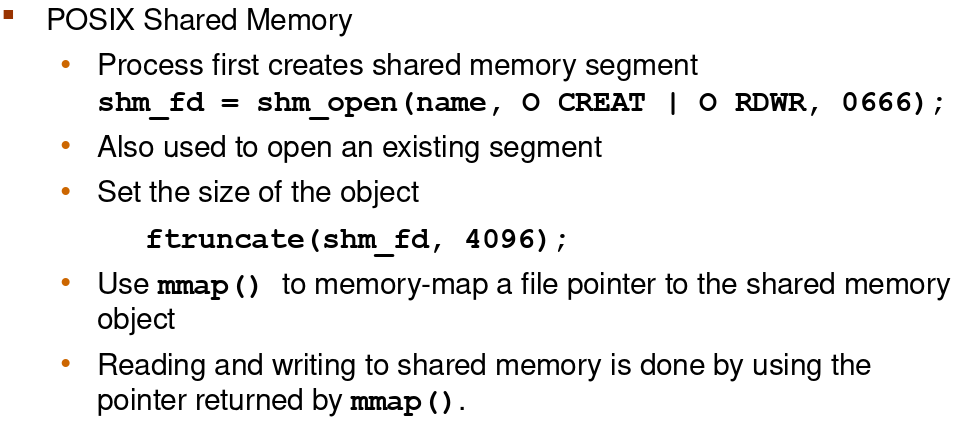
\includegraphics[scale=0.3]{7_sharedmem.png}
\end{center}

\subsection*{Mach}
\paragraph*{Message based}
\begin{enumerate}
    \item syscallurile sunt mesaje
    \item toate taskurile au 2 porturi la creare: kernel si notify
    \item mesajele sunt trimise si primite cu mach\_msg()
    \item portul e creat cu mach\_port\_allocate()
    \item send si receive sunt flexibile, 4 optiuni daca mailboxul e full
          \begin{enumerate}
              \item asteapta nedefinit
              \item asteapta max n ms
              \item returneaza imediat
              \item cachuieste un mesaj temporar
          \end{enumerate}
\end{enumerate}

\subsection*{Pipes}
\paragraph*{Comunicare intre 2 procese}
\subsection*{Ordinary pipes}
\paragraph*{Nu pot fi accesate din afara procesului care le-a creat}
\begin{enumerate}
    \item Comunicare standard in stil producer-consumer
    \item Producerul: write-end of the pipe
    \item Consumerul: read-end of the pipe
    \item Unidirectionale
    \item Au nevoie de parent-child
\end{enumerate}

\subsection*{Named pipes}
\paragraph*{Pot fi accesate fara relatie parent-child}
\begin{enumerate}
    \item Comunicarea e bidirectionoala
    \item Nu e nevoie de parent-child
    \item Mai multe procese pot folosi acelasi pipe
\end{enumerate}

\subsection*{Sistemele client-server}
\paragraph*{Sockets}
\begin{enumerate}
    \item endpoint de comunicare
    \item IP:PORT
    \item <1024 well known
    \item 127.0.0.1 loopback
\end{enumerate}
\paragraph*{RPC}
\begin{enumerate}
    \item Abstractizeaza procedura callurilor dintre procese si sistemele din retea
    \item foloseste porturi
    \item stubs - client-side proxy pentru procedura actuala din server
    \item stubul localizeaza serverul si marshalls parametrii
    \item server-side stub primeste mesajul, dezpacheteaza parametrii si face procedura
    \item reprezentarea datelor se face prin XDL (External Data Representation)
    \item comunicarea are mai multe failure scenarios (mesajele pot fi trimise o SINGURA data sau CEL MULT o data)
    \item OS-ul are un rendezvous (sau matchmaker) service ca sa conecteze clientul si serverul
\end{enumerate}

\section[Ch4 Threads and Concurrency]{Threads and Concurrency}
\paragraph*{Beneficii}
\begin{enumerate}
    \item Responsivness - continuarea executiei daca o parte din proces e blocata (UI)
    \item Resource Sharing - partajeaza cu procesele mai usor ca shared memory sau message passing
    \item Economie - mai ieftin decat crearea proceselor, iar threa switching mai ieftin ca message passing
    \item Scalabilitate - procesele pot folosi arhitecturile multicore
\end{enumerate}

\paragraph*{Paralelism} - un sistem poate face mai mult de 1 lucru simultan
\paragraph*{Concurrency} - sustine mai mult de un task care face progres (single processor/core - scheduler providing concurrency)

\paragraph*{Tipuri de paralelism}
\begin{enumerate}
    \item Data paralelism - distribuie submultimi ale datelor pe mai multe coreuri, aceeasi operatie pentru fiecare
    \item Task parallelism - distribuie threadurile pe coreuri, fiecare thread facand o actiune unica
\end{enumerate}

\paragraph*{Legea lui Amdahl}

\begin{center}
    \begin{math}
        speedup \leq \frac{1}{S+\frac{(1-S)}{N}}
    \end{math}
\end{center}

\subparagraph*{title} S = portiunea seriala, N = numarul de coreuri

\paragraph*{User vs Kernel Threads}

\subsection*{Modele multithreading}
\begin{enumerate}
    \item Many-to-One
    \item One-to-One
    \item Many-to-Many
\end{enumerate}

\paragraph*{Many-to-one}
\begin{enumerate}
    \item Mai multe threaduri user-level mapate pe un thread de kernel
    \item Un thread blocking le face pe toate sa se blocheze
    \item Mai multe threaduri pot sa nu ruleze in paralel pe un sistem multicore pentru ca numai unul poate fi in kernel la un moment dat
    \item Exemple: Solaris Green Threads, GNU Portable Threads
\end{enumerate}
\paragraph*{One-to-One}
\begin{enumerate}
    \item Fiecare thread user-level mapeaza pe un thread al kernelului
    \item Crearea unui thread la user level creaza un thread in kernel
    \item Mai multa concurenta decat many-to-one
    \item Numarul de threaduri pe proces restrictionat din cauza overheadului
\end{enumerate}
\paragraph*{Many-to-Many}
\begin{enumerate}
    \item Mai multe user level threads mapate pe mai multe kernel threads
    \item Sistemul poate crea un numar suficient de threaduri de kernel
    \item Exemplu (necomun): ThreadFiber pe Windows
\end{enumerate}
\paragraph*{Two-level Model} Ca M:M, doar ca un user thread poate fi bound catre un kernel thread

\begin{center}
    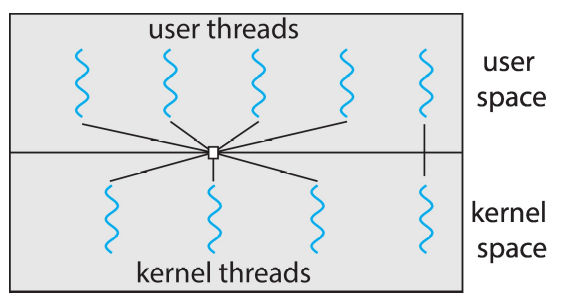
\includegraphics[scale=0.3]{8_twolevelmodel.png}
\end{center}

\subsection*{Pthreads}
\begin{enumerate}
    \item User-level sau kernel-level
    \item Un API POSIX standard pentru crearea si sincronizarea threadurilor
    \item Specificatie, nu implementare
    \item API-ul specifica comportamentul librariei, nu al implementarii
    \item Comun in UNIX
\end{enumerate}

\begin{center}
    \begin{lstlisting}
#include <errno.h>
#include <pthread.h>
#include <stdio.h>
#include <stdlib.h>
#include <string.h>

void* rev_str(void* v)
{
    int len = strlen((char*)v);

    char* rev = malloc(sizeof(char) * (len + 1));
    rev[len] = '\0';

    char* p = (char*)v;

    do {
        rev[len - 1] = *p++;
    } while(--len);


    return rev;
}

int main(int argc, char** argv)
{
    pthread_t thr;
    void* res;
    if (argc < 2) {
        printf("Usage: %s <string> \n", argv[0]);
        return -1;
    }

    if (pthread_create(&thr, NULL, rev_str, argv[1])) {
        perror(NULL);
        return errno;
    }

    if (pthread_join(thr, &res)) {
        perror(NULL);
        return errno;
    }
    printf("%s\n", (char*)res);
    return 0;
}
    \end{lstlisting}
\end{center}

\subsection*{Implicit threading}
\begin{enumerate}
    \item Thread Pools
    \item Fork-Join
    \item OpenMP
    \item Grand Central Dispatch
    \item Intel Threading BUilding Blocks
\end{enumerate}

\paragraph*{Thread Pools} Creaza un numar de threaduri intr-o piscina unde asteapta munca
\begin{enumerate}
    \item De obicei ceva mai rapide sa preia un request cu unul existent decat cu crearea unuia nou
    \item Nr de threaduri maxim marimea poolului
    \item Separarea taskurilor de mecanismele de creare a taskurilor permit diferite strategii de run (ex: periodical schedule)
\end{enumerate}

\paragraph*{Fork-join Parallelism} Mai mult threaduri sunt forkuite, apoi joinate

\begin{center}
    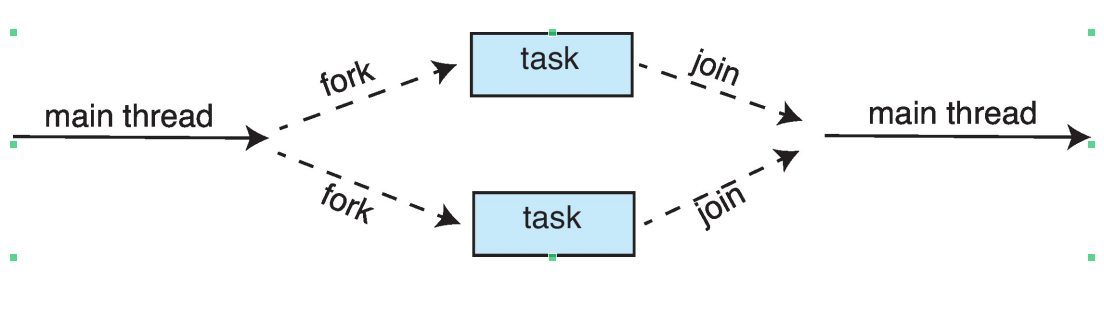
\includegraphics[scale=0.3]{9_forkjoin.png}
\end{center}

\subparagraph*{Algoritmul general}
\begin{center}
    \begin{lstlisting}
Task(problem){
    if (problem is small enough){
        solve directly;
    } else {
        subtask1 = fork (new Task (subset of problem));
        subtask2 = fork (new Task (subset of problem));

        result1 = join(subtask1);
        result2 = join(subtask2);

        return combined results;
    }
}
    \end{lstlisting}
\end{center}

\begin{center}
    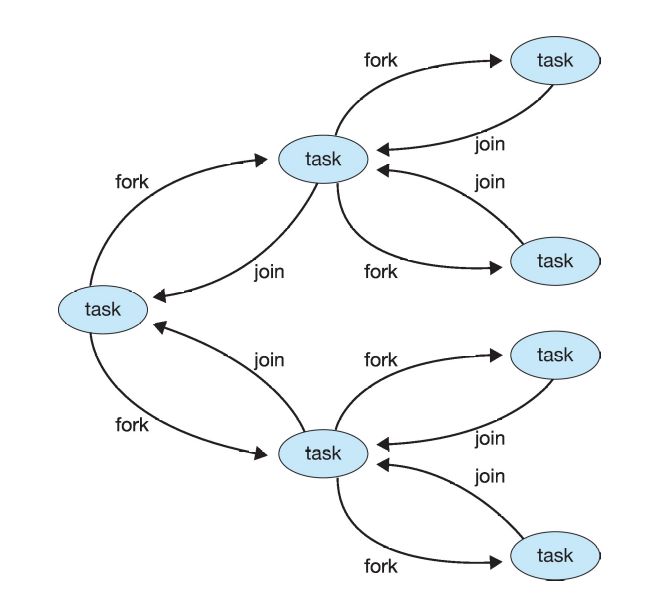
\includegraphics[scale=0.3]{10_forkjoin.png}
\end{center}

\paragraph*{OpenMP}
\begin{enumerate}
    \item O multime de directive de compilator si un API pentru C, C++, FROTRAN
    \item Suport pentru programarea paralela in mediile cu shared-memory
    \item Identifica regiunile paralele (blocheaza codul paralel)
    \item Se creaza threaduri pe cat de multe coreuri sunt
\end{enumerate}

\paragraph*{Grand Central Dispatch}
\begin{enumerate}
    \item Apple technology for macOS and iOS
    \item Extensii C, C++ si Objective-C, API si librarie run-time
    \item Permite identificarea sectiunilor paralele
    \item Gestioneaza majoritatea detaliilor in threading
    \item Blocul este intre \^\ \{\}
    \item Blocurile sunt puse in dispatch queue si sunt asignate unui thread disponibil din pool cand sunt scoase din coada
    \item Doua tipuri de dispatch queues
          \begin{enumerate}
              \item serial - FIFO, queue per proces, numit main queue
              \item concurent - FIFO, dar mai multe o data
          \end{enumerate}
\end{enumerate}

\subsection*{Threading issues}
\paragraph*{Semantica fork() si exec()}
\subparagraph*{Fork()} de obicei duplica doar calling thread (Linux), dar pe alte sisteme, toate threadurile
\subparagraph*{Exec()} de obicei inlocuieste procesul care ruleaza inclusiv threadurile sale

\paragraph*{Signal handling} folosit pentru procesarea semnalelor
\begin{enumerate}
    \item Semnal generat de un anumit eveniment
    \item Semnalul este dat unui proces
    \item Semnalul este ahndeluit de 1 din cele doua handleluri
          \begin{enumerate}
              \item default
              \item user-defined
          \end{enumerate}
\end{enumerate}

\paragraph*{Thread Cancellation} Terminarea unui thread (numit si target thread) inainte de sfarsit
\subparagraph*{2 metode:} Asincrona (imediata), Deferred (target threadul verifica periodic daca trebuie cancelat). Tipul implicit e deferred. Pe Linux thread cancellation e obtinut prin semnale

\paragraph*{TLS (Thread Local Storage)} permite fiecarui thread sa aiba copia proprie a datelor si e folositor la thread pooluri (unde nu ai control asupra crearii)

\subsection*{Scheduler Activations}
M:M si Two-level au nevoie de comunicare pentru a aloca numarul potrivit de threaduri de Kernel. De obicei se foloseste o structura de date intermediara intre threadurile de user si de kernel LWP (lightweight process). Acesta apare ca un procesor virtual unde procesele pot face scheduleing pentru rularea user threadurilor, fiecare LWP e atasat unui thread de kernel. Scheduler activations au upcalls (un mecanism de comunicare de la kernel la upcall handler)

\subsection*{Linux threads}
\begin{enumerate}
    \item Li se zice tasks
    \item Se fac prin syscallul clone()
    \item clone() permite taskurilor copil sa partajeze address space-ul parintelui (procesului)
\end{enumerate}

\section[Ch5 CPU Scheduling]{CPU Scheduling}
\paragraph*{CPU - I/O Burst cycle} un ciclu de cpu execution si I/O wait

\begin{center}
    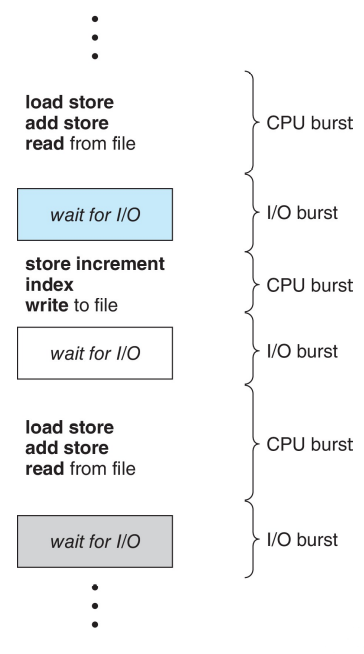
\includegraphics[scale=0.3]{11_cpuioburstcycle.png}
\end{center}

\subsection*{CPU Scheduler} Selecteaza din procesele din queue (ordonata in moduri diferite) si aloca un core de CPU unuia
\subparagraph*{Deciziile pot avea loc atunci cand:}
\begin{enumerate}
    \item Running $\rightarrow$ waiting
    \item Running $\rightarrow$ ready
    \item Waiting $\rightarrow$ ready
    \item Terminates
\end{enumerate}
\subparagraph*{Optiuni:} Pentru 1 \& 4 \textbf{NU} exista, pentru 2 \& 3 exista. Asadar pentru 1 \& 4 este nonpreemptive (o data alocat, procesul pastreaza CPU-ul pana se termina sau se schimba la waiting), altfel este preemptive.
\subparagraph*{Preemptive} poate duce la race conditions

\subsection*{Dispatcher}
\paragraph*{Dispatcher-ul} da controlul CPU-ului procesului selectat de \textbf{scheduler}. Acest lucru inseamna: schimbarea de context, schimbarea in user mode, jump la locatia din programul userului pentru a restarta programul
\paragraph*{Dispatch latency} - timpul care ii ia dispatcher-ului sa opreasca un proces, apoi sa ruleze altul

\subsection*{Scheduling criteria}
\paragraph*{WT} = ultimul timp de inceput al procesului - suma tuturor timpilor anteriori de sfarsit - arrival time
\begin{enumerate}
    \item \textbf{CPU utilizations} - sa fie cat mai ocupat
    \item \textbf{Throughput} - nr de procese care isi completeaza executia per unitate de timp
    \item \textbf{Turnaround time} - timpul de executie al unui proces
    \item \textbf{Waiting time} - timpul pe care un proces l-a petrecut in ready queue
    \item \textbf{Response time} - timpul pe care un proces il petrece de cand a facut o cerere pana cand primul raspuns este produs
\end{enumerate}

\subsection*{FCFS (First-Come, First-Served)}
\paragraph*{Convoy effect} - short process behind long process
\begin{center}
    \begin{tabularx}{0.8\textwidth} {
            | >{\centering\arraybackslash}X
            | >{\centering\arraybackslash}X
            |}
        \hline
        Process & Burst Time \\
        \hline
        $P_1$   & 24         \\
        $P_2$   & 3          \\
        $P_3$   & 3          \\
        \hline
    \end{tabularx}
\end{center}

\begin{center}
    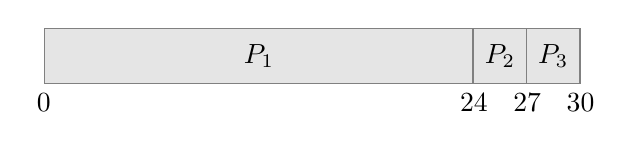
\begin{tikzpicture}[node distance=-0.5pt]
        \node [gray box=24] (p1) {\(P_{1}\)};
        \node [gray box=3, right=of p1] (p2) {\(P_{2}\)};
        \node [gray box=3, right=of p2] (p3) {\(P_{3}\)};

        \node [annotation] at (p1.south west) {0};
        \node [annotation] at (p1.south east) {24};
        \node [annotation] at (p2.south east) {27};
        \node [annotation] at (p3.south east) {30};
    \end{tikzpicture}
\end{center}
\paragraph*{Waiting time:} $P_1 = 0$; $P_2 = 24$; $P_3 = 27$
\paragraph*{Average waiting time:} $\frac{(0+24+27)}{3} = 17$

\subsection*{SJF (Shortest-Job-First)}
\paragraph*{SJF e optim} - are media timpurilor de asteptare pentru o multime de procese ca fiind minima
\paragraph*{Shortest-remaining-time-first} este numele versiunii preemptive

\begin{center}
    \begin{tabularx}{0.8\textwidth} {
            | >{\centering\arraybackslash}X
            | >{\centering\arraybackslash}X
            |}
        \hline
        Process & Burst Time \\
        \hline
        $P_1$   & 6          \\
        $P_2$   & 8          \\
        $P_3$   & 7          \\
        $P_4$   & 3          \\
        \hline
    \end{tabularx}
\end{center}

\begin{center}
    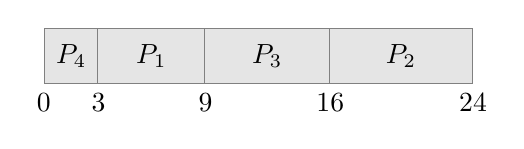
\begin{tikzpicture}[node distance=-0.5pt]
        \node [gray box=3] (p4) {\(P_{4}\)};
        \node [gray box=6, right=of p4] (p1) {\(P_{1}\)};
        \node [gray box=7, right=of p1] (p3) {\(P_{3}\)};
        \node [gray box=8, right=of p3] (p2) {\(P_{2}\)};

        \node [annotation] at (p4.south west) {0};
        \node [annotation] at (p4.south east) {3};
        \node [annotation] at (p1.south east) {9};
        \node [annotation] at (p3.south east) {16};
        \node [annotation] at (p2.south east) {24};
    \end{tikzpicture}
\end{center}

\paragraph*{Average waiting time:} $\frac{(3+16+9+0)}{4} = 7$

\paragraph*{Cum determinam lungimea CPU burst?}
\subparagraph*{Estimare:} ar trebui sa fie asemanatoare cu cele anterioare. Poate fi folosita cu exponential averaging
\begin{enumerate}
    \item $t_n$ = lungimea reala a celui de-al n-ulea CPU burst
    \item $\tau_{n+1}$ = valoarea prezisa pentru urmatorul CPU burst
    \item $\alpha,0 \leq \alpha \leq 1$ (de obicei e setat la $\frac{1}{2}$)
    \item Definim: $\tau_{n+1} = \alpha t_n + (1-\alpha) \tau_{n}$
\end{enumerate}

\subsection*{Shortest Remaning Time First}
\paragraph*{SJN} - versiunea preemtiva. Cand ajunge in coada de ready, decizia de a-l programa urmatorul este refacuta cu alogirtmul SJN

\begin{center}
    \begin{tabularx}{0.8\textwidth} {
            | >{\centering\arraybackslash}X
            | >{\centering\arraybackslash}X
            | >{\centering\arraybackslash}X
            |}
        \hline
        Process & Arrival Time & Burst Time \\
        \hline
        $P_1$   & 0            & 8          \\
        $P_2$   & 1            & 4          \\
        $P_3$   & 2            & 9          \\
        $P_4$   & 3            & 5          \\
        \hline
    \end{tabularx}
\end{center}

\begin{center}
    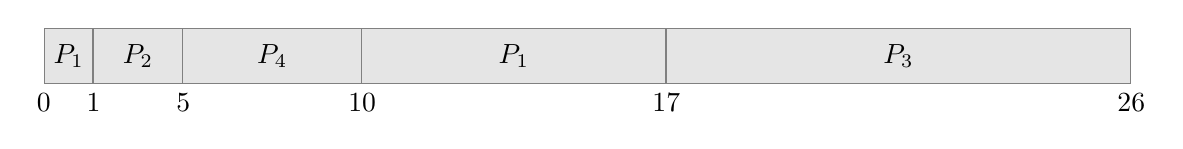
\begin{tikzpicture}[node distance=-0.3pt]
        \node [gray box=1] (p1) {\(P_{1}\)};
        \node [gray box=5, right=of p1] (p2) {\(P_{2}\)};
        \node [gray box=10, right=of p2] (p4) {\(P_{4}\)};
        \node [gray box=17, right=of p4] (p11) {\(P_{1}\)};
        \node [gray box=26, right=of p11] (p3) {\(P_{3}\)};

        \node [annotation] at (p1.south west) {0};
        \node [annotation] at (p1.south east) {1};
        \node [annotation] at (p2.south east) {5};
        \node [annotation] at (p4.south east) {10};
        \node [annotation] at (p11.south east) {17};
        \node [annotation] at (p3.south east) {26};
    \end{tikzpicture}
\end{center}

\begin{center}
    \begin{tabularx}{0.8\textwidth} {
            | >{\centering\arraybackslash}X
            | >{\centering\arraybackslash}X
            | >{\centering\arraybackslash}X
            | >{\centering\arraybackslash}X
            |}
        \hline
        Process & Completion Time & Turnaround Time (CT-AT) & Waiting time (TAT-BT) \\
        \hline
        $P_1$   & 17              & 17                      & 9                     \\
        $P_2$   & 5               & 4                       & 0                     \\
        $P_3$   & 26              & 24                      & 15                    \\
        $P_4$   & 10              & 7                       & 2                     \\
        \hline
    \end{tabularx}
\end{center}

\paragraph*{Average waiting time:} $[9+0+15+2]/4 = 26/4 = 6.5$

\subsection*{Round Robin (RR)}
\begin{enumerate}
    \item Fiecare proces ia o unitate mica de timp pe CPU (\textbf{time quantum} $q$), de obicei intre 10-100 ms. Dupa aceast timp, procesul este preempted si adaugat la sfarsitul queueului de ready
    \item Daca sunt n procese si time quantum este q, atunci ficare proces ia bucati de $\frac{1}{n}$ din timpul CPU-ului de cel mult q unitati de timp o data. Niciun proces nu asteapta mai mult de $(n-1)q$ unitati de timp
    \item Exista un timer care intrerupe fiecare quantum pentru scheduleing pe noul proces
    \item Performanta:
          \begin{enumerate}
              \item q mare $\approx$ FIFO(FCFS)
              \item q mic $\approx$ RR
          \end{enumerate}
\end{enumerate}

\begin{center}
    \begin{tabularx}{0.8\textwidth} {
            | >{\centering\arraybackslash}X
            | >{\centering\arraybackslash}X
            |}
        \hline
        Process & Burst Time \\
        \hline
        $P_1$   & 24         \\
        $P_2$   & 3          \\
        $P_3$   & 3          \\
        \hline
    \end{tabularx}
\end{center}

\begin{center}
    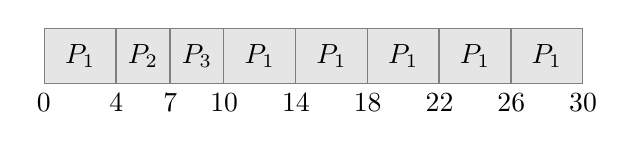
\begin{tikzpicture}[node distance=-0.3pt]
        \node [gray box=4] (p1) {\(P_{1}\)};
        \node [gray box=3, right=of p1] (p2) {\(P_{2}\)};
        \node [gray box=3, right=of p2] (p3) {\(P_{3}\)};
        \node [gray box=4, right=of p3] (p11) {\(P_{1}\)};
        \node [gray box=4, right=of p11] (p112) {\(P_{1}\)};
        \node [gray box=4, right=of p112] (p111) {\(P_{1}\)};
        \node [gray box=4, right=of p111] (p1111) {\(P_{1}\)};
        \node [gray box=4, right=of p1111] (p11111) {\(P_{1}\)};

        \node [annotation] at (p1.south west) {0};
        \node [annotation] at (p1.south east) {4};
        \node [annotation] at (p2.south east) {7};
        \node [annotation] at (p3.south east) {10};
        \node [annotation] at (p11.south east) {14};
        \node [annotation] at (p112.south east) {18};
        \node [annotation] at (p111.south east) {22};
        \node [annotation] at (p1111.south east) {26};
        \node [annotation] at (p11111.south east) {30};
    \end{tikzpicture}
\end{center}
\begin{center}
    \textbf{A fost folosit time quantum = 4}
\end{center}

\paragraph*{De obicei $TAT \ge SJF$, dar raspuns mai bun}
\paragraph*{q trebuie sa fie mai mare decat timpul de context switch.} De obicei q intre 10ms si 100ms, iar context switch $\le 10 \mu s$

\subsection*{Priority Scheduling}
\paragraph*{Priority number} - integer asociat fiecarui proces (nr mic - prioritate mare)
\paragraph*{SJF} este un priority scheduling unde prioritatea este inversul timpului urmator de CPU burst prezis
\paragraph*{Problema} Starvation $\Rightarrow$ \textbf{Solutie} Aging

\begin{center}
    \begin{tabularx}{0.8\textwidth} {
            | >{\centering\arraybackslash}X
            | >{\centering\arraybackslash}X
            | >{\centering\arraybackslash}X
            |}
        \hline
        Process & Burst Time & Priority \\
        \hline
        $P_1$   & 10         & 3        \\
        $P_2$   & 1          & 1        \\
        $P_3$   & 2          & 4        \\
        $P_4$   & 1          & 5        \\
        $P_5$   & 5          & 2        \\
        \hline
    \end{tabularx}
\end{center}

\begin{center}
    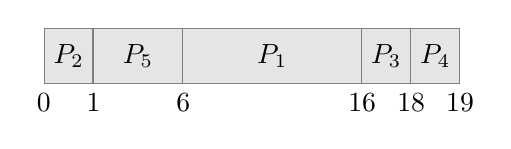
\begin{tikzpicture}[node distance=-0.3pt]
        \node [gray box=1] (p2) {\(P_{2}\)};
        \node [gray box=5, right=of p2] (p5) {\(P_{5}\)};
        \node [gray box=10, right=of p5] (p1) {\(P_{1}\)};
        \node [gray box=2, right=of p1] (p3) {\(P_{3}\)};
        \node [gray box=1, right=of p3] (p4) {\(P_{4}\)};

        \node [annotation] at (p2.south west) {0};
        \node [annotation] at (p2.south east) {1};
        \node [annotation] at (p5.south east) {6};
        \node [annotation] at (p1.south east) {16};
        \node [annotation] at (p3.south east) {18};
        \node [annotation] at (p4.south east) {19};
    \end{tikzpicture}
\end{center}

\paragraph*{Priority Scheduling cu Round-Robin (time quantum = 2)}
\begin{center}
    \begin{tabularx}{0.8\textwidth} {
            | >{\centering\arraybackslash}X
            | >{\centering\arraybackslash}X
            | >{\centering\arraybackslash}X
            |}
        \hline
        Process & Burst Time & Priority \\
        \hline
        $P_1$   & 4          & 3        \\
        $P_2$   & 5          & 2        \\
        $P_3$   & 8          & 2        \\
        $P_4$   & 7          & 1        \\
        $P_5$   & 3          & 3        \\
        \hline
    \end{tabularx}
\end{center}

\begin{center}
    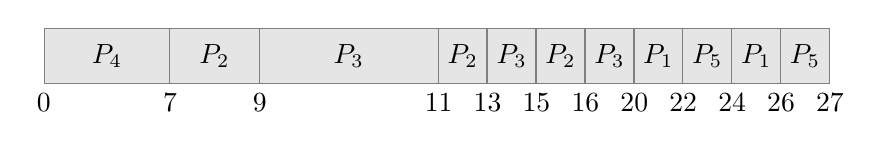
\begin{tikzpicture}[node distance=-0.3pt]
        \node [gray box=7] (p4) {\(P_{4}\)};
        \node [gray box=5, right=of p4] (p2) {\(P_{2}\)};
        \node [gray box=10, right=of p2] (p3) {\(P_{3}\)};
        \node [gray box=2, right=of p3] (p2i) {\(P_{2}\)};
        \node [gray box=1, right=of p2i] (p3i) {\(P_{3}\)};
        \node [gray box=1, right=of p3i] (p2ii) {\(P_{2}\)};
        \node [gray box=1, right=of p2ii] (p3ii) {\(P_{3}\)};
        \node [gray box=1, right=of p3ii] (p1) {\(P_{1}\)};
        \node [gray box=1, right=of p1] (p5) {\(P_{5}\)};
        \node [gray box=1, right=of p5] (p1i) {\(P_{1}\)};
        \node [gray box=1, right=of p1i] (p5i) {\(P_{5}\)};

        \node [annotation] at (p4.south west) {0};
        \node [annotation] at (p4.south east) {7};
        \node [annotation] at (p2.south east) {9};
        \node [annotation] at (p3.south east) {11};
        \node [annotation] at (p2i.south east) {13};
        \node [annotation] at (p3i.south east) {15};
        \node [annotation] at (p2ii.south east) {16};
        \node [annotation] at (p3ii.south east) {20};
        \node [annotation] at (p1.south east) {22};
        \node [annotation] at (p5.south east) {24};
        \node [annotation] at (p1i.south east) {26};
        \node [annotation] at (p5i.south east) {27};
    \end{tikzpicture}
\end{center}

\subsection*{Multilevel Queue}
\begin{enumerate}
    \item Numarul de queues
    \item Algoritmul de scheduling pentru fiecare queue
    \item Meoda de determinare a queue-ului in care procesul intra
    \item Scheduling intre queues
\end{enumerate}

\begin{center}
    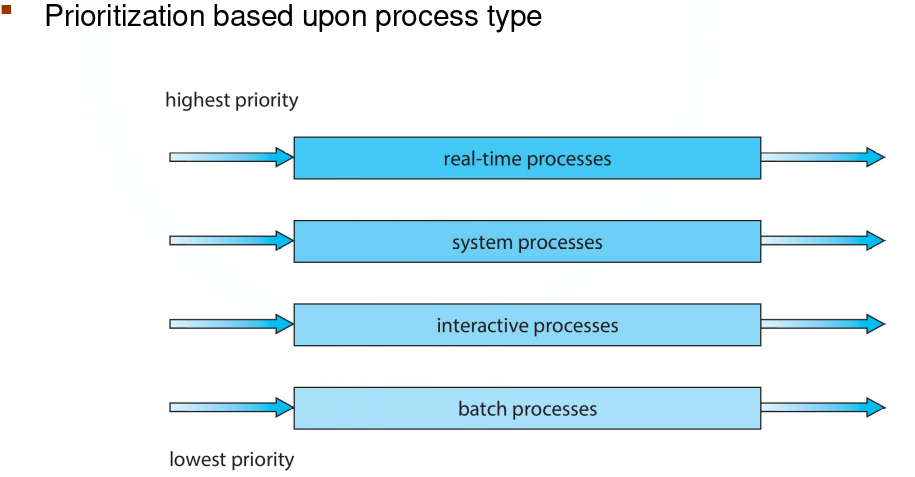
\includegraphics[scale=0.3]{12_mqproctype.png}
\end{center}

\subsection*{Multilevel Feedback Queue}
\paragraph*{}Un proces se poate misca prin queues diferite
\begin{enumerate}
    \item Numarul de cozi
    \item Algoritmul de scheduling pentru fiecare coada
    \item Metoda de determinare a upgradarii procesului
    \item Metoda de determinare a demote procesului
    \item Metoda de determinare a cozii in care un proces intra
    \item Aging poate fi implementat folosind multilevel feedback queue
\end{enumerate}

\subsection*{Thread Scheduling}

\begin{center}
    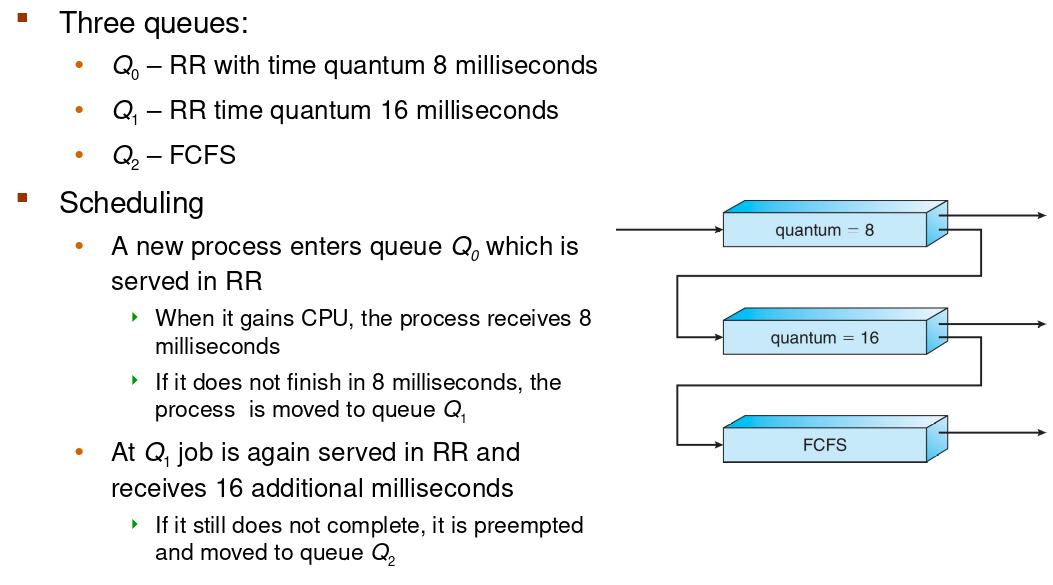
\includegraphics[scale=0.3]{13_exmq.png}
\end{center}

\begin{enumerate}
    \item Distinctie intre user-level si kernel-level threads
    \item Cand threadurile sunt suportate, ele sunt scheduluite, nu procesele
    \item \textbf{PCS} - process-contention scope pentru ca schdedulingul e facut per proces de obicei prin prioritate data de programator
    \item Kernel thread scheduling este denumit si \textbf{SCS} system-contention scope pentru ca intra in competitie cu celelalte threaduri din sistem
\end{enumerate}

\paragraph*{Pthread scheduling} API-ul permite PCS sau SCS, dar pe Linux si macOS  doar \textbf{pthread\_scope\_system}

\subsection*{Multiple-Processor Scheduling}
\paragraph*{Poate fi}
\begin{enumerate}
    \item CPU multicore
    \item Multithreaded cores
    \item NUMA systems
    \item Multiprocesare eterogena
\end{enumerate}
\paragraph*{SMP} - symmetric multiprocessing unde fiecare procesor face self scheduling fie prin common ready queue fie prin cozi private de threaduri pe ficare procesor
\paragraph*{Multithreaded multicore system} - Fiecare core are $> 1$ threaduri hardware. Daca exista memory stall pe un thread, face switch la altul
\subparagraph*{CMT} - chip-multithreading (Intel ii zice hyperthreading)
\subparagraph*{Sunt 2 nivele:}
\begin{enumerate}
    \item OS decide ce software thread sa ruleze pe fiecare CPU
    \item Fiecare core decide ce hardware thread sa ruleze pe core-ul fizic
\end{enumerate}
\subparagraph*{Load balancing} pentru a tine workloadul distribuit uniform se fac \textbf{push migrations} (de a lua de la un cpu overloaded la altul) si \textbf{pull migrations} (procesoarele idle preiau taskuri de la cele ocupate)
\subparagraph*{Processor affinity} - cand un thread ruleaza pe un procesor, cacheul acelui procesor tine memoria accesata de thread fie prin \textbf{soft affinity} (OS-ul incearca fara garantii) sau \textbf{hard affinity} (permite unui proces sa specifice o multime de procesoare pe care sa ruleze). Load balancingul poate afecta processor affinity.

\paragraph*{NUMA-aware} inseamna ca va asigna memoria apropiata de CPU-ul pe care ruleaza

\paragraph*{Real-Time CPU Scheduling} pe sistemele \textbf{soft real-time} face ca taskurile real-time sa aiba prioritate mare, dar nu garanteaza ca vor fi schedeluite, iar pe cele \textbf{hard real-time} taskurile trebuie sa fie facute pana la deadline.
\subparagraph*{2 tipuri de latenta} afecteaza performata: \textbf{interrupt latency}, timpul de la sosirea interruptului la startul rutinei care serveste interruptul, \textbf{dispatch latency}, timpul pe care se scurge de la luarea procesului curent de pe CPU si schimbarea cu altul.

\paragraph*{Priority based-scheduling} pentru real-time scheduling trebuie sa suporte scheduling preemptive si priority-based, dar garanteaza numai soft real-time. Pentru hard real-time trebuie sa aiba abilitatea de a intruni deadlineurile.
\subparagraph*{Periodic} - cere CPU la intervale constante. Pnetru timpul de procesare t, deadlineul d si perioada p ($0\leq t \leq d \leq p$) rata taskului periodic este $\frac{1}{p}$

\paragraph*{Rate monotonic scheduling} - perioadele scurte au prioritate mare, cele lungi, prioritate mica. Se poate intampla ca un proces sa rateze deadlineul.
\paragraph*{EDF (earliest deadline first scheduling)} - prioritatile se asigneaza in functie de deadlineuri (devereme - prioritate mare, tarziu - prioritate mica)
\paragraph*{Proportional share scheduling} sunt T shares pentru toate procesele. O aplicatie primeste N shares ($N < T$) astfel incat sa primeasca $N/T$ din timpul total de procesor.
\paragraph*{POSIX Real-Time Scheduling} are un api cu 2 clase de scheduling
\begin{enumerate}
    \item SCHED\_FIFO - cu strategia FCFS si coada FIFO. Fara time-slicing pentru threaduri cu prioritate egala
    \item SCHED\_RR - la fel ca prima, dar exista time-slicing pentru threaduri cu prioritate egala
\end{enumerate}


\subsection*{Linux scheduling}
\paragraph*{Pana la 2.5} avea variatii ale algoritmului de scheduling standard din UNIX. De la 2.5 s-a mutat in timp constant O(1).
\begin{enumerate}
    \item Preemptive, priority based
    \item 2 rangeuri de prioritati: time-sharing si real-time
    \item real-time intre 0 si 99 si nice value de la 100 la 140
    \item Taskul este runable cat timp mai are timp in time slice (active)
    \item Daca nu mai are timp (expired) nu mai este runable pana cand celelalte taskuri isi folosesc sliceurile
    \item Toate taskurile runable sunt tinute per-CPU in runqueue
          \begin{enumerate}
              \item 2 arrayuri de proritate (active, expired)
              \item taskuri indexate pe prioritate
              \item cand nu mai sunt active, arrayurile se schimba
          \end{enumerate}
    \item A mers bine, dar poor response times pentru procesele interactive
\end{enumerate}
\paragraph*{De la 2.6.23} se foloseste \textbf{CFS} (Completely Fair Scheduler) care introduce \textbf{clase}:
\begin{enumerate}
    \item Fiecare are prioritate specifica
    \item Schedulerul se uita dupa taskul cu prioritate maxima in clasa cu prioritate maxima
    \item In loc de quantum based, e bazat pe proportia din CPU time
    \item 2 incluse (altele pot fi adaugate): default, real-time
    \item Quantumul e calculat pe nice value de la -20 la +19 si calculeaza target latency (intervalul in care fiecare task trebuie sa ruleze macar 1 data)
    \item Tine virtual run time per task (vruntime) si alege taskul cu cel mai mic virtual runtime
    \item Tine totul intr-un red-black tree
    \item Nice de -20 e prioritate globala de 100 si +19 de 139
\end{enumerate}

\begin{center}
    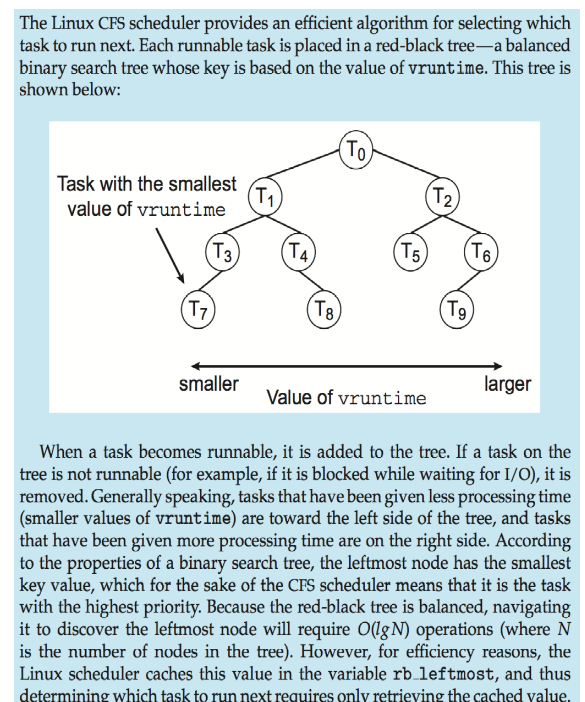
\includegraphics[scale=0.4]{13_cfs.png}
\end{center}

\paragraph*{Linux scheduling} suporta load balancing, dar este si NUMA-aware, grupand multimile de coreuri de CPU care pot fi in balanta intr-un scheduling domain

\subsection*{Selectarea algoritmului de evaluare}
\paragraph*{Determinist} cu evaluare analitica
\paragraph*{Formula lui Little}
\begin{enumerate}
    \item n = average queue length
    \item W = average waiting time in queue
    \item $\lambda$ = average arrival rate into queue
    \item $ n = \lambda * W$
\end{enumerate}
\paragraph*{Simulari} dar au accuracy limitat

\section[Ch6 Synchronization Tools]{Synchronization Tools}
\subsection*{Critical section problem}
\paragraph*{Procesele} trebuie sa ceara permisiune de intrare in critical section in \textbf{entry section}, pot continua cu \textbf{exit section}, apoi cu \textbf{remainder section}.
\paragraph*{Requirements}
\begin{enumerate}
    \item Mutula exclusion - daca $P_i$ este in critical section, niciun alt proces nu mai poate executa cod de acolo
    \item Progress - daca niciun proces nu executa din critical section si exista procese care cer acces, acest lucru nu poate fi amanat pe termen nedeterminat
    \item Bounded waiting - exista o limitare a numarului de dati in care alte procese pot intra in critical section pana ca un proces care a facut cererea de a intra este lasat sa o faca
\end{enumerate}
\paragraph*{Solutia 1.} Pentru 2 procese. Presupunem ca load si store sunt instructiuni machine-language atomice care shareuiesc o variabila \textbf{int turn}. Initial turn are valoarea i.
\begin{lstlisting}
while(true){
    while(turn == j);

    /* critical section */
    turn = j;
    /* remainder section */
}
\end{lstlisting}
\subparagraph*{Mutual exclusion} e pastrat, nu si progress requirement sau bounded-waiting requirement.
\paragraph*{Solutia lui Peterson.} 2 procese. La fel cu load si store sunt atomice. Au 2 variabile \textbf{int turn; boolean flag[2];}. Turn spune cui ii este randul, flag spune daca un proces e gata sa intre in critical section.

\begin{lstlisting}
while(true){
    flag[i] == true;
    turn = j;
    while(flag[j] && turn == j);

    /* critical section */
    flag[i] = false;
    /* remainder section */
}
\end{lstlisting}
\subparagraph*{Cele 3 CS requirements sunt indeplinite.} Mutual exclusion, progress requirement si bounded-waiting requirement. Totusi, pentru multithreaded poate produce rezultate neasteptate.

\begin{center}
    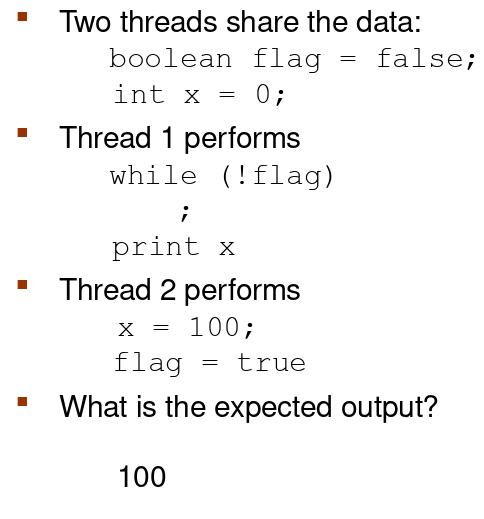
\includegraphics[scale=0.3]{14_peterson2threads.png}
\end{center}
\subparagraph*{Reordonarea} celor 2 instructiuni din Threadul 2 se poate intampla pentru ca flag si x sunt independente, asa ca outputul poate fi 0.

\begin{center}
    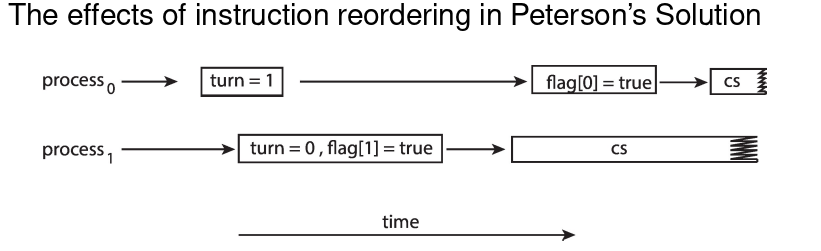
\includegraphics[scale=0.4]{15_ptersonrevisited.png}
\end{center}
\subparagraph*{Memory Barrier} e folosit pentru acest caz astfel incat sa nu intre ambele procese in critical section.

\subsection*{Memory barrier}
Garantiile pe care arhitectura calculatoarelor le face pentru programe.
\begin{enumerate}
    \item Strongly ordered - o modificare a memoriei pe un procesor e imediat vizibila si celorlalte procesoare
    \item Weakly ordered - nu e imediat vizibila
\end{enumerate}
\paragraph*{Memory barrier} - o instructiune care foteaza orice modificare in memorie sa fie propagata si celorlalte procesoare.

\begin{center}
    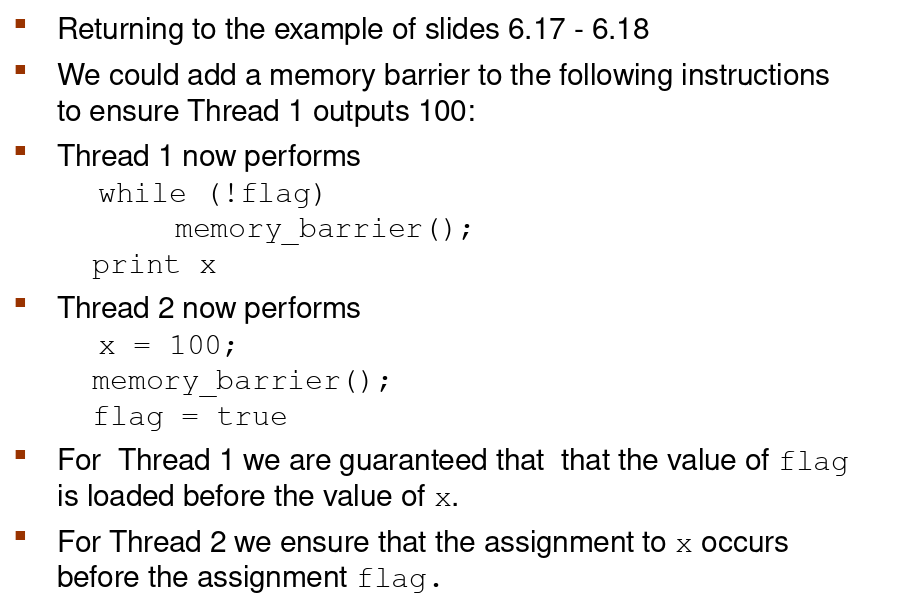
\includegraphics[scale=0.3]{16_membarrier.png}
\end{center}


\subsection*{Synchronization Hardware}
\begin{enumerate}
    \item Uniprocessors - executa codul running fara preemption, dar sunt ineficiente si OS-urile care folosesc asta nu sunt scalabile
    \item Hardware instructions
    \item Atomic variables
\end{enumerate}

\paragraph*{Hardware instructions} - test-and-set sau compare-and-swap atomice
\begin{lstlisting}
boolean test_and_set (boolean *target){
    boolean rv = *target;
    *target = true;
    return rv;
}
\end{lstlisting}
\begin{enumerate}
    \item Se executa atomic
    \item Returneaza valoarea originala a parametrului
    \item Seteaza noua valoare a parametrului ca true
\end{enumerate}

\begin{lstlisting}
do {
    while(test_and_set(&lock)); /* do nothing */
    /* cs */
    lock = false;
    /* remainder section */
} while (true);
\end{lstlisting}

\begin{lstlisting}
int compare_and_swap (int *value, int expected, int new_value){
    int temp = *value;
    if (*value == expected)
        *value = new_value;
    return temp;
}
\end{lstlisting}
\begin{enumerate}
    \item Executat atomic
    \item Returneaza valoarea originala din value
    \item Seteaza value cu new\_value, numai daca *value == expected
\end{enumerate}

\begin{lstlisting}
while(true){
    while(compare_and_swap(&lock, 0, 1) != 0); /* do nothing */
    /* cs */
    lock = 0;

    /* remainder section */
}
\end{lstlisting}

\paragraph*{Bounded-waiting cu compare-and-swap}\
\begin{lstlisting}
while(true){
    waiting[i] = true;
    key = 1;
    while(waiting[i] && key == 1)
        key = compare_and_swap(&lock, 0 ,1);
    waiting[i] = false;
    /* cs */
    j = (i+1) % n;
    while((j!=i) && !waiting[j])
        j = (j+1) % n;
    if(j == i)
        lock = 0;
    else
        waiting[j] = false;
    /* remainder section */
}
\end{lstlisting}

\paragraph*{Atomic variables}
Presupunem ca sequence e o variabila atomica, iar increment() este o operatie atomica pe sequence. Asadar increment(\&sequence) face ca sequence sa fie incrementat fara intrerupere.

\begin{center}
    \begin{lstlisting}
void increment(atomic_int *v){
    int temp;
    do{
        temp = *v;
    } while(temp!= (compare_and_swap(v, temp, temp+1)));
}
    \end{lstlisting}
\end{center}

\paragraph*{Mutex locks} Sunt ceva mai simple. Protejeaza cs cu acquire() si realease() care sunt atomice (de obice instructiuni hardware atomice cum ar fi compare-and-swap). Foloseste \textbf{busy waiting}, de aceea lockul se numeste \textbf{spinlock}

\begin{center}
    \begin{lstlisting}
while(true){
    /* acquire lock */
        /* cs */
    /* release lock */
    /* remainder section */
}
    \end{lstlisting}
\end{center}

\paragraph*{Semaphore} Mai sofisticat decat mutex locks. Semaforul S este integer si poate fi accesat via 2 operatii atomice wait() si signal()

\begin{center}
    \begin{lstlisting}
wait(S){
    while(S <= 0); // busy wait
    S--;
}
    \end{lstlisting}
\end{center}
\begin{center}
    \begin{lstlisting}
signal(S){
    S++;
}
    \end{lstlisting}
\end{center}
\subparagraph*{Pot fi 2:} counting sempahore (integer peste un domeniu nerestrictionat) sau binary semaphore (intre 0 si 1, asemanator cu un mutex lock). Un counting sempahore poate fi implementat ca un binary semaphore.

\subparagraph*{Waiting queue} asociat cu fiecare semafor. Fiecare item are value (integer) si pointer (catre urmatorul item). Se fac 2 operatii: block (procesul care invoca operatia este bagat in coada) si wakeup (scoate din waiting queue procesul si il pune in ready queue). Asa se poate face fara busy waiting.
\begin{center}
    \begin{lstlisting}
typdef struct{
    int value;
    struct process *list;
} semaphore;

wait(semaphore *S){
    S->value--;
    if(S->value < 0){
        adauga la S->list;
        block();
    }
}

signal(semaphore *S){
    S->value++;
    if(S->value <= 0){
        scoate P din S->list;
        wakeup(P);
    }
}
    \end{lstlisting}
\end{center}

\paragraph*{Monitors} Hihg-level abstraction. Numai 1 procesor poate fi activ cu un monitor la un moment dat
\begin{center}
    \begin{lstlisting}
monitor monitor-name{
    // shared variable declarations
    procedure P1(...){...}
    procedure P2(...){...}

    procedure Pn(...){...}

    initialization code(...) {...}
}
    \end{lstlisting}
\end{center}

\subparagraph*{Implementarea de monitoare cu semafoare.} Variabilele \textbf{semaphore mutex; mutex = 1;}. Fiecare procedura P va avea structura:
\begin{center}
    \begin{lstlisting}
wait(mutex);
        ...
        body of P;
        ...
signal(mutex);
    \end{lstlisting}
\end{center}

\paragraph*{Condition variables.} condition x,y; Sunt 2 operatii: x.wait() si x.signal(). Ultima rezuma procesul care a invocat.
\subparagraph*{Folosire} Consideram $P_1$ si $P_2$ care trebuie sa execute $S_1$ si $S_2$ (statementuri) astfel incat $S_1$ sa se intample inainte de $S_2$. Cream un monitor cu doua proceduri $F_1$ invocata de $P_1$ si $F_2$ invocata de $P_2$. O variabila conditionala x initializata cu 0. O variabila booleana \textbf{done}.

\begin{center}
    \begin{lstlisting}
F1:
        S1;
        done=true;
        x.signal();
F2:
        if done == false
            x.wait()
        S2;
    \end{lstlisting}
\end{center}

\paragraph*{Implementare monitoare cu semafoare}
\subparagraph*{Variabile:}
\begin{center}
    \begin{lstlisting}
semaphore mutex; // initial 1
semaphore next; // initial 0
int next_count = 0; // numarul de procese in waiting in monitor
    \end{lstlisting}
\end{center}

\subparagraph*{Fiecare functie P va fi }
\begin{center}
    \begin{lstlisting}
wait(mutex);
        ...
        body of P;
        ...
if(next_count > 0)
        signal(next);
else
        signal(mutex);
    \end{lstlisting}
\end{center}

\paragraph*{Implementare de condition variables}
\subparagraph*{Fie x} condition variable avem:
\begin{center}
    \begin{lstlisting}
semaphore x_sem; // initial 0
int x_count = 0;
    \end{lstlisting}
\end{center}
\subparagraph*{x.wait()}
\begin{center}
    \begin{lstlisting}
x_count++;
if(next_count > 0)
        signal(next);
else
        signal(mutex);
wait(x_sem);
x_count--;
    \end{lstlisting}
\end{center}
\subparagraph*{x.signal()}
\begin{center}
    \begin{lstlisting}
if(x_count > 0){
    next_count++;
    signal(x_sem);
    wait(next);
    next_count--;
}
    \end{lstlisting}
\end{center}

\paragraph*{Rezumarea proceselor dintr-un monitor} Daca mai multe procese au facut coada in condition variable x, atunci ce se executa dupa x.signal()? FCFS nu e adecvat. Se foloseste \textbf{conditional-wait} sub forma x.wait(c). C este un integer (numar de prioritate).

\paragraph*{Single Resource allocation}
\begin{center}
    \begin{lstlisting}
R.acquire(t);
        ...
        access the resource;
        ...
R.release;
    \end{lstlisting}
\end{center}
\paragraph*{Monitor pentru alocarea single resource}
\begin{center}
    \begin{lstlisting}
monitor ResourceAllocator 
{ 
    boolean busy; 
    condition x; 
    void acquire(int time) { 
        if (busy) 
            x.wait(time); 
        busy = true; 
    } 
    void release() { 
        busy = false; 
        x.signal(); 
    } 
    initialization code() {
        busy = false; 
    }
}		
\end{lstlisting}
\end{center}
\subsection*{Liveness}
\paragraph*{Liveness} se refera la faptul ca un sistem trebuie sa obtina progres pe procese. Waiting indefinit este liveness failure
\paragraph*{Deadlock} - 2 sau mai multe procese asteapta nedefinit pentru un eveniment care poate fi cauzat doar de unul dintre cele din coada de waiting

\begin{center}
    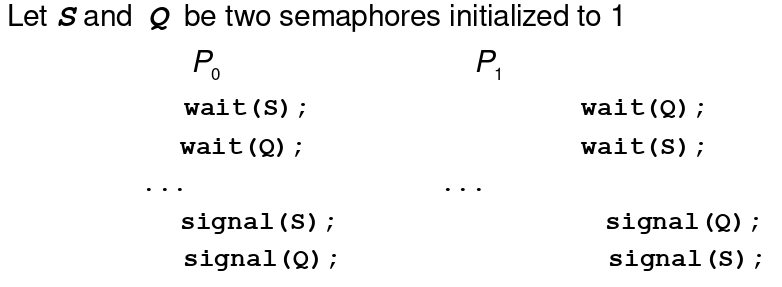
\includegraphics[scale=0.4]{16_deadlock.png}
\end{center}

\subparagraph*{Alte forme de deadlock:} starvation (indefinite blocking - un proces poate sa nu fie scos niciodata din semaphore queue), priority inversion - cand un proes cu lower-priority are un lock necesar unui proces cu higher-priority (rezolvat prin priority-inheritance protocol).


\section[Ch7 Synchronization Examples]{Synchronization Examples}


\subsection*{Bounded-buffer problem}
\begin{center}
    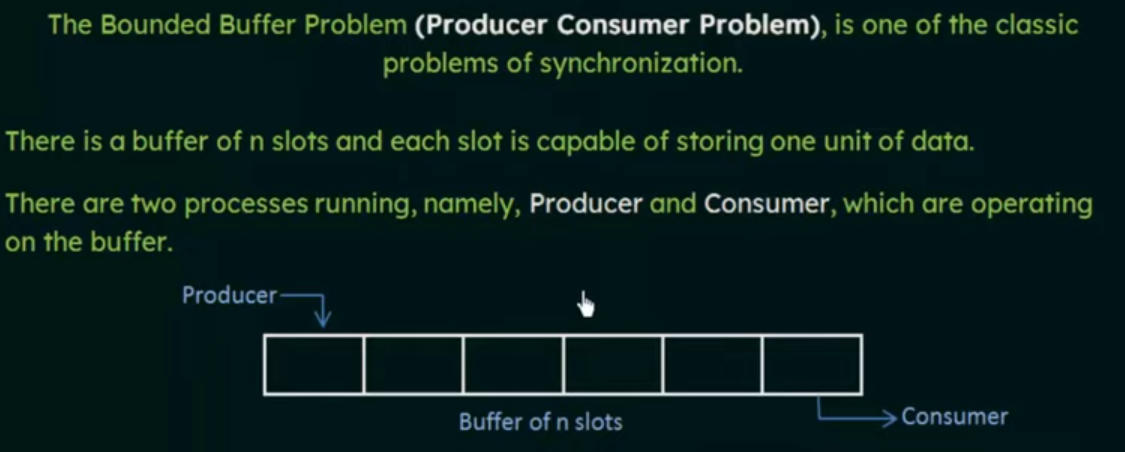
\includegraphics[scale=0.3]{17_boundedbuffer.png}
\end{center}
\begin{enumerate}
    \item \textbf{n} buffere au un hold pe un item
    \item semaforul \textbf{mutex} este initializat cu 1 - binar, folosit ca sa faca acquire si release pe lock
    \item semaforul \textbf{full} este intializat cu 0 - cate sloturi sunt folosite in buffer
    \item semaforul \textbf{empty} este initializat cu valoarea n - nr de sloturi din buffer
\end{enumerate}
\paragraph*{Structura prcesului producer}
\begin{center}
    \begin{lstlisting}
while (true) { 
    ...
    /* produce an item in next_produced */ 
    ... 
    wait(empty);  // wait until empty > 0, then decrement empty
    wait(mutex);  // acquire the lock
        ...
    /* add next produced to the buffer */ 
        ... 
    signal(mutex); // release the lock
    signal(full); // increment full
}
    \end{lstlisting}
\end{center}
\paragraph*{Structura procesului consumer}
\begin{center}
    \begin{lstlisting}
while (true) { 
    wait(full); // wait until full > 0 and decrement full
    wait(mutex); // acquire lock
        ...
    /* remove an item from buffer to next_consumed */ 
        ... 
    signal(mutex); // release lock
    signal(empty); // increment empty
        ...
    /* consume the item in next consumed */ 
        ...
    }
    \end{lstlisting}
\end{center}

\subsection*{Readers-Writers Problem}
\paragraph*{Un data set} este shareuit intre mai multe procese concurente. Unele sunt \textbf{Readers} care pot doar citi, altii sunt \textbf{Writers} care pot citi si scrie. Problema: permite ca mai multi readeri sa citeasca in acelasi timp, iar 1 singur writer poate accesa data in acelasi timp.

\subparagraph*{Shared data}
\begin{enumerate}
    \item Data Set
    \item semaforul rw\_mutex initializat cu 1 - comun intre readeri si writeri
    \item semaforul mutex initializat cu 1 - mutual exclusion cand read\_count e actualizat (cand readerii intra sau ies din cs)
    \item integer reader\_count initializat cu 0 - cate procese citesc din data set
\end{enumerate}

\subparagraph*{Writer}
\begin{center}
    \begin{lstlisting}
while (true) {
    wait(rw_mutex);  // request cs
            ...
    /* writing is performed */ 
            ... 
    signal(rw_mutex); // leaves cs
}
    \end{lstlisting}
\end{center}

\subparagraph*{Reader}
\begin{center}
    \begin{lstlisting}
while (true){
    wait(mutex); // lock pentru read_count
    read_count++; // increase the number of readers by 1
    if (read_count == 1) /* first reader */ 
            wait(rw_mutex); // no writer can enter if there is even 1 reader
            signal(mutex); // other readers can enter while the current reader is inside the cs
        ...
    /* reading is performed */ 
        ... 
    wait(mutex);
    read_count--; // a reader wants to leave
    if (read_count == 0) /* last reader */
        signal(rw_mutex); // writers can enter
    signal(mutex); // reader leaves
}
    \end{lstlisting}
\end{center}

\paragraph*{Probleme.} Aceasta rezolvare e numita "first reader-writer problem" pentru ca poate rezulta intr-un writer care sa nu scrie niciodata. "Second reader-writer problem" e o variatie care spune ca "O data ce un writer e gata sa scrie, niciun reader nou nu poate fi lasat sa citeasca". Ambele pot rezulta in starvation. Problema este rezolvata in unele sisteme prin reader-writer locks in kernel.

\subsection*{Dining-Philosophers Problem}
\begin{enumerate}
    \item N filozifi stau la o masa rotunda cu un castron de orez la mijloc
    \item Ei alterneaza intre mancat si gandit
    \item Nu interactioneaza cu vecinii
    \item Uneori incearca sa ia 2 chopstickuri (cate unul pe rand). Au nevoie de 2 ca sa manance si le dau release cand termina.
    \item Shared data: castronul cu orez (data set), semaforul chopstick[n] initializat cu 1
\end{enumerate}

\paragraph*{Solutia cu semafoare.} Filosoful i:
\begin{center}
    \begin{lstlisting}
while (true){ 
    wait (chopstick[i] );
    wait (chopStick[ (i + 1) % n] ); // N are nevoie de (n-1) si 0

    /* eat for a while */

    signal (chopstick[i] );
    signal (chopstick[ (i + 1) % n] );

    /* think for a while */

}
    \end{lstlisting}
\end{center}
\subparagraph*{Deadlock} Ne asigura ca nu exista 2 vecini care sa manance simultan, dar tot poate crea deadlock. Sa zicem ca toti filosofii vor sa manance in acelasi timp, asta inseamna ca toate elementele din chopstick[n] vor fi 0, dar cand fiecare filosof vrea sa ia chopstickul din dreapta va astepta la nesfarsit.
\subparagraph*{Remedii deadlock}
\begin{enumerate}
    \item Tacamuri pentru n, dar numai n-1 filosofi
    \item Un filosof ar trebui sa poata lua ambele chopstickuri numai daca ambele sunt disponibile (trebuie sa le ia in cs)
    \item Solutie asimetrica: impar ia mai intai stanga, apoi dreapta, iar par mai intai dreapta, apoi stanga
\end{enumerate}

\paragraph*{Solutia cu monitoare}
\subparagraph*{Restrictie:} un filosof poate sa ia chopstickurile, numai daca ambele sunt disponibile
\begin{center}
    \begin{lstlisting}
monitor DiningPhilosophers
{ 
    /* cele 3 stateuri in care un filosof se poate afla */
    enum {THINKING; HUNGRY, EATING} state [5]; 
    condition self [5];

    void pickup (int i) { 
            state[i] = HUNGRY;
            test(i); // verifica vecinii daca mananca
            /* Daca nu e eating in urma testului, asteapta semnalul altora care vine din putdown */
            if (state[i] != EATING)
                self[i].wait;
    }
    
    void putdown (int i) { 
            /* Isi schimba statusul */
            state[i] = THINKING;
                    // test left and right neighbors
            /* Cheama test pe vecini pentru ca si ei sa poata sa manance */
            test((i + 4) % 5); // vecinl din stanga
            test((i + 1) % 5); // vecinul din dreapta
    }
    void test (int i) { 
        /* Daca in stanga nu mananca, in dreapta nu mananca si actualul e hungry */
        if (
            (state[(i + 4) % 5] != EATING) &&
            (state[i] == HUNGRY) &&
            (state[(i + 1) % 5] != EATING) 
        ) { 
            /* Mananca */
            state[i] = EATING;

            /* A terminat de mancat si spune ca pot veni si altii */
            self[i].signal();
        }
    }

   initialization_code() { 
       for (int i = 0; i < 5; i++)
       state[i] = THINKING;
     }
}

/* Asa se servesc filosofii */
DiningPhilosophers.pickup(i);

    /** EAT **/

DiningPhilosophers.putdown(i);
    \end{lstlisting}
\end{center}

\subparagraph*{Starvation} e posibil, dar nu are deadlock

\subsection*{Transactional Memory}
\paragraph*{Memory transaction} e o secventa de operatii read-write atomica.

\subparagraph*{Cu mutex locks}
\begin{center}
    \begin{lstlisting}
void update(){
    acquire();

    /* modify shared data */

    release();
}
    \end{lstlisting}
\end{center}

\subparagraph*{Cu memory transaction}
\begin{center}
    \begin{lstlisting}
void update(){
    atomic{
        /* modify shared data */
    }
}
    \end{lstlisting}
\end{center}

\subsection*{OpenMP}
\paragraph*{} O multime de directive de compilator si API care suporta programarea paralela.

\begin{center}
    \begin{lstlisting}
void update(int value)
{
    /* codul de mai jos e tratat ca un cs si facut atomic */
    #pragma omp critical
    {
        count += value
    }
}
    \end{lstlisting}
\end{center}

\subsection*{Limbaje functionale}
\begin{enumerate}
    \item Limbajele de PF au o alta paradigma, aceea ca nu mentin stateul
    \item Variabilele sunt imutabile si nu isi pot schimba stateul o data ce au avut asignata o valoare
    \item Au o abordare mai interesanta a data races
\end{enumerate}

\section[Ch9 Main memory]{Main memory}
\subsection*{Protection}
Un proces trebuie sa acceseze numai adresele din spatiul lui de adrese. Se pot adauga registri de \textbf{base} si \textbf{limit}.
\paragraph*{Hardware Address Protection} - CPU-ul trebuie sa verifice daca fiecare acces de memorie generat in user mode este intre base si base + limit.
\subsection*{Address Binding}
Programele de pe disc care sunt gata de a fi aduse in memroie sunt executate ca un \textbf{input queue}.
\paragraph*{Reprezentarea adreselor}
\begin{enumerate}
    \item Codul sursa foloseste de obicei adrese simbolice
    \item Codul compilat binduieste catre adrese relocabile
    \item Linkerul sau loaderul va bindui adresele relocabile la adrese aboslute
    \item Fiecare binding mapeaza un address space catre altul
\end{enumerate}
\paragraph*{Momentele din timp in care se binduiesc instructiunile si data in memorie}
\begin{enumerate}
    \item Compile time - daca adresa de memorie e cunoscuta a priori, poate fi generat \textbf{absolute code}
    \item Load time - trebuie sa genereze \textbf{relocatable code} daca locatia de memorie nu e cunoscuta la compilare
    \item Execution time - bindigul e amanat pana la run time daca procesul poate fi mutat in timpul executiei dintr-un segment de memorie in altul (e nevoie de suport hardware pentru address maps)
\end{enumerate}

\subsection*{Logical vs Physical Address Space}
\paragraph*{Logical address} - generata de CPU, cunoscuta si ca \textbf{virtual address}
\paragraph*{Physical address} - adresa vazuta de unitatea de memorie
\paragraph*{Adresele logice si fizice} sunt aceleasi la compile-time si load-time, dar difera la execution-time

\paragraph*{Logical address space} - multimea tuturor adreselor logice generate de un program
\paragraph*{Physical address space} - multimea tuturor adreselor fizice generate de un program

\subsection*{MMU (Memory Management Unit)}
Dispozitivul hardware care mapeaza adresele virtuale catre cele fizice. Sunt posibile mai multe metode.
\paragraph*{Un caz simplu (generalizarea base-register scheme): }  base register e acum numit \textbf{relocation register}. Valoarea din relocation register e adaugata catre toate adresele generate de un proces in momentul in care este trimis in memorie. Programul userului lucreaza cu adrese logice si nu le vede pe cele reale fizice. Are loc execution-time bindig cand referinta este facuta la o locatie din memorie, iar adresele logice sunt legate de cele fizice.

\begin{center}
    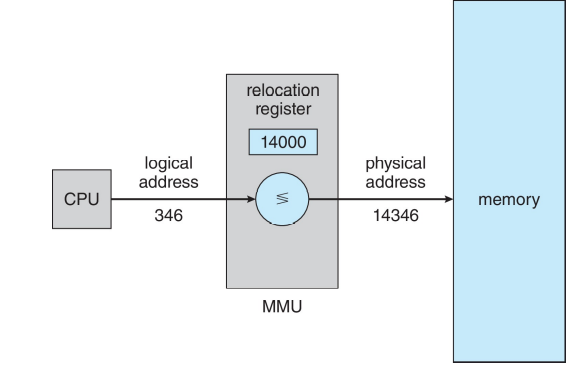
\includegraphics[scale=0.4]{18_mmu.png}
\end{center}

\paragraph*{Dynamic Loading}
\begin{enumerate}
    \item Nu tot programul trebuie sa fie in memorie ca sa fie executat
    \item Rutinile nu sunt incarcate pana nu sunt apelate
    \item Utilizare mai buna a memory-space
    \item Toate rutinele sunt tinute pe disc in relocatable load format
    \item Folositor cand bucati mari de cod sunt necesare pentru a gestiona cazuri rare
    \item Nu e nevoie de suport special din partea OS (se implementeaza prin designul programului, dar OS-ul poate ajuta prin librarii care sa implementeze dynamic loading)
\end{enumerate}

\paragraph*{Dynamic Linking}
\begin{enumerate}
    \item Static linking - librariile si codul programului combinate de loader intr-o imagine binara a programului
    \item Dynamic linking - linkingul amanat pana la execution tim
    \item Stub - o bucata mica de cod care localizeaza rutina necesara din libraria ce rezida in memorie si apoi se inlocuieste cu adresa rutine si o executa
    \item OS verifica daca rutina este in adresa de memorie a programului (daca nu e in address space, o adauga)
    \item Dynamic linking e folositoare pentru librarii
    \item Sistemul e cunoscut ca \textbf{shared libraries}
    \item Pentru patchingul librariilor e nevoie de versionare
\end{enumerate}

\paragraph*{Contiguous Allocation}
\begin{enumerate}
    \item Main memory trebuie sa suport atat OS-ul cat si procesele utilizatorului
    \item Resurse limitate, trebuie alocate eficient
    \item E o metoda incipienta
    \item Imparte main memory in 2 partitii
          \begin{enumerate}
              \item Resident operating system (low memory cu interrupt vector)
              \item User processes (high memory, fiecare proces cu o zona continua de memorie)
          \end{enumerate}
    \item Registrii de relocare protejeaza procesele userilor unul de altul si de schimbarea codului si datelor OS-ului
          \begin{enumerate}
              \item Base register contine valoarea celei mai mici adrese fizice
              \item Limit register contine un range de adrese logice (fiecare adresa logica trebuie sa fie mai mica decat el)
              \item MMU mapeaza adresele logice dinamic
              \item Poate suport codul kernelului sa fie transient si kernelul sa isi schimbe dimensiunile
          \end{enumerate}
\end{enumerate}

\paragraph*{Variable partitions}
\begin{enumerate}
    \item Multiprogramming limitat de numarul de partiti
    \item Marimi variabile pentru eficienta
    \item Hole - bloc de memorie disponibil, gaurile de memorie sunt imprastiate prin intreg sistemul
    \item Cand vine un proces, i se acorda loc dintr-o gaura suficient de mare ca sa incapa
    \item Exit - paritita se elibereaza, iar partiile libere adiacente se combina
    \item OS tine informatii despre
          \begin{enumerate}
              \item Partitii alocate
              \item Partitii libere (hole)
          \end{enumerate}
\end{enumerate}

\paragraph*{Dynamic storage-allocation problem}
\begin{enumerate}
    \item First fit - aloca prima gaura suficient de mare
    \item Best fit - aloca cea mai mica gaura suficient de mare (trebuie sa caute in intraga lista daca nu este ordonata dupa marime)
    \item Worst fit - aloca cea mai mare gaura (la fel trebuie sa caute in intreaga lista)
\end{enumerate}

\paragraph*{Fragmentare}
\subparagraph*{Fragmentare externa} - spatiul total de memorie exista ca sa satisfaca o cerere, dar nu e continuu
\subparagraph*{Fragmentare interna} - memoria alocata poate fi un pic mai mare decat cea ceruta, diferenta fiind interna unei partitii, dar nefiind folosita
\subparagraph*{Analiza first fit} poate da N blocuri alocate, dar 0.5 N sunt pierdute fragmentarii (1/3 pot fi neutilizabile $\rightarrow$ 50-percent rule)
\subparagraph*{Compaction} - metoda de a reduce fragmentarea externa. Se aranjeaza memoria astfel incat toata memoria libera sa fie impreuna intr-un bloc mare. Compactarea e posibila numai daca relocarea e dinamica si se face la execution time. Poate aparea problem I/O (leaga un job in memorie cat timp este implicat in I/O sau fa I/O in buffere de OS)

\subsection*{Paging}
Spatiul de adresare fizic al unui proces poate fi necontinuu, iar procesului ii poate fi alocata memorie fizica atunci cand are nevoie sau este disponibila.
\begin{enumerate}
    \item Se protejeaza impotriva fragmentarii si a bucatilor de memorie de marimi variabile
    \item \textbf{Frames} - memoria fizica e divizata in blocuri fixe de marimea puterilor lui 2
    \item \textbf{Pages} - la fel dar pe memoria logica
    \item Pentru un program de N pagini, trebuie N frameuri libere
    \item Se face un page table care sa traduca adresele logice in fizice
    \item Backing store impartit in pagini
    \item Inca exista fragmentare interna
\end{enumerate}

\paragraph*{Address translation scheme}
Adresa generata de CPU este impartita in:
\begin{enumerate}
    \item page number (p) - un index intr-un \textbf{page table} care contine adresa base a fiecarei pagini in memoria fizica
    \item page offset (d) - combinat cu adresa de baza pentru a defini adresa de memorie fizica care este trimisa unitatii de memorie
\end{enumerate}

\begin{center}
    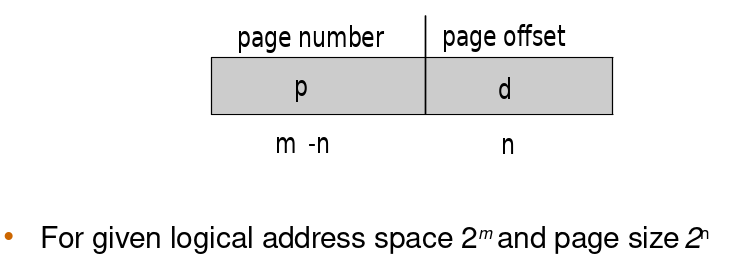
\includegraphics[scale=0.4]{19_pages.png}
\end{center}

\paragraph*{Calculul internal fragmentation}

\begin{enumerate}
    \item Page size = 2,048 bytes
    \item Process size = 72,766 bytes
    \item 35 pages + 1,086 bytes
    \item Internal fragmentation of 2,048 - 1,086 = 962 bytes
    \item Worst case fragmentation = 1 frame - 1 byte
    \item On average fragmentation = 1 / 2 frame size
    \item So small frame sizes desirable?
    \item But each page table entry takes memory to track
    \item Page sizes growing over time
          \begin{enumerate}
              \item Solaris supports two page sizes - 8 KB and 4 MB
          \end{enumerate}
\end{enumerate}

\paragraph*{Implementarea page table}
\begin{enumerate}
    \item PTBR (page-table base register) - pointeaza catre page table
    \item PTLR (page-table length register) - indica marimea paginii tabelului
    \item Cele 2 probleme de acces pot fi rezolvate prin \textbf{TLBs} (translation-look-aside buffers) numite si \textbf{memorie asociativa}
\end{enumerate}

\paragraph*{TLB} - unele stocheaza \textbf{ASIDs} (address-space identifiers) in fiecare TLB entry ca sa identifice in mod unic fiecare proces pentru a-i oferi address-space protection.
\subparagraph*{Marimea} este de obicei mica (64 - 1024 intrari)
\subparagraph*{TLB miss} - valoarea e incarcata in TLB pentru acces rapid data viitoare. Trebuie implementate politici de inlocuire. Unele intrari trebuie sa fie incastrate pentru acces permanent rapid

\begin{center}
    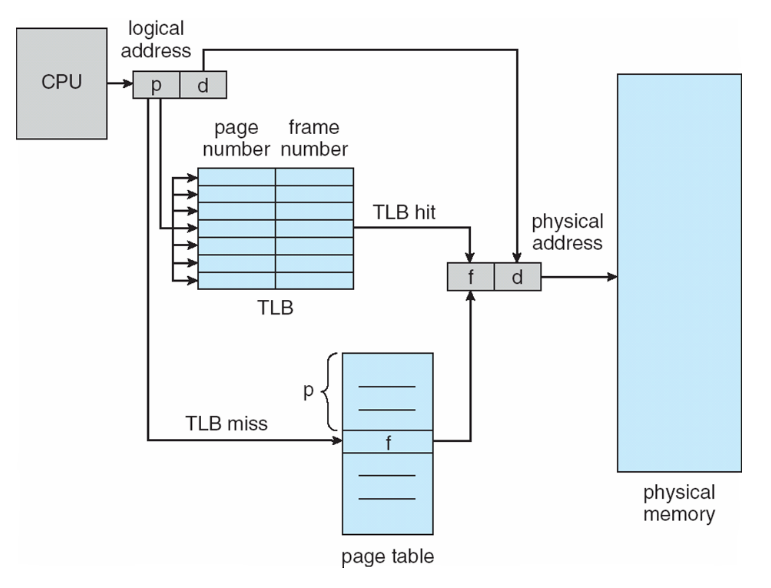
\includegraphics[scale=0.4]{20_tlbhardware.png}
\end{center}

\paragraph*{Effective Access Time} - hit ratio este procentul in care pagina e gasita in TLB
\subparagraph*{Exemplu:} 10ns pentru acces la memorie. Daca nu e in TLB, se fac 2 accesari, adica 20ns. $EAT=0.80*10+0.20*20=12$

\paragraph*{Memory protection} - poate fi implementata asociind un bit de protectie cu fiecare frame ca sa indice daca accesul read-only sau write-only este permis. De fapt, pot fi mai multi biti care sa indice page execute-only etc.
\subparagraph*{Valid-invalid bit} - atasat fiecarei intrari din page table, unde valid inseamna ca se afla in logical address space-ul procesului, deci e pagina legala, iar invalid altfel. Sau se foloseste \textbf{PTLR} (page-table length register). Orice incalcare determina un trap in kernel

\subsection*{Shared Pages}
\paragraph*{Shared Code} - doar o copie a codului read-only (reentrant) e shareuit intre procese. De asemenea pentru IPC e folositor sa fie shareuite si read-write pages.
\subparagraph*{Private code and data} - fiecare proces are o copie separata a codului si datelor, fiecare pagina pentru private code and data poate aparea oriunde in logical address space

\subsection*{Structure of the Page Table}
\begin{enumerate}
    \item Hierarchical Paging
    \item Hashed Page Tables
    \item Inverted Page Tables
\end{enumerate}

\paragraph*{Hierarchical Page Tables}
\begin{enumerate}
    \item Imparte logical address space in mai multe pagini
    \item O tehnica simpla e sa avem mai page table pe 2 nivele
\end{enumerate}

\begin{center}
    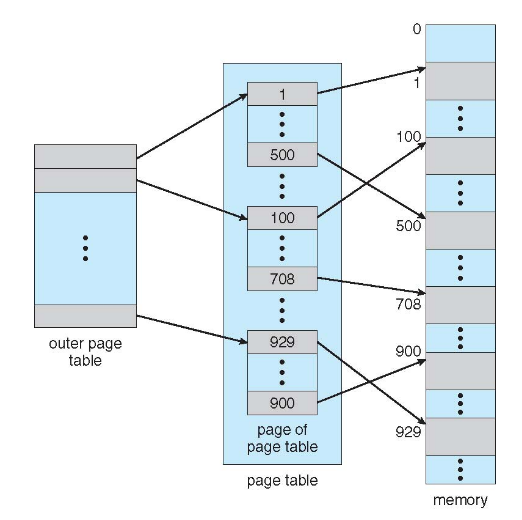
\includegraphics[scale=0.3]{21_hpt.png}
\end{center}

\subparagraph*{2-level paging}
\begin{enumerate}
    \item O adresa logica pe 32biti are 4k si este divizata intr-un page number cu 20bits si page offset cu 12 bits
    \item Din moment ce page tablelul e paged, page number e divizat in: 10bit page number si 10 bit offset
\end{enumerate}
\subparagraph*{Forward-mapped page table} $p_1$ este indexul catre outer page table, $p_2$ este displacementul in interiorul paginii pentru inner page table si $d$ este page offsetul

\begin{center}
    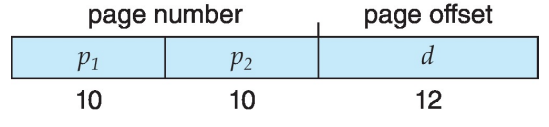
\includegraphics[scale=0.3]{22-fmpt.png}
\end{center}

\subparagraph*{Address-Translation scheme}
\begin{center}
    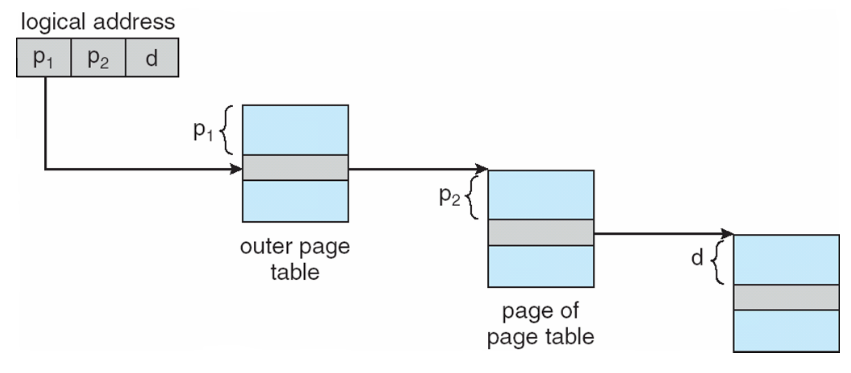
\includegraphics[scale=0.3]{23-ats.png}
\end{center}

\subparagraph*{3-level paging scheme pe 64bits}
\subparagraph*{Address-Translation scheme}
\begin{center}
    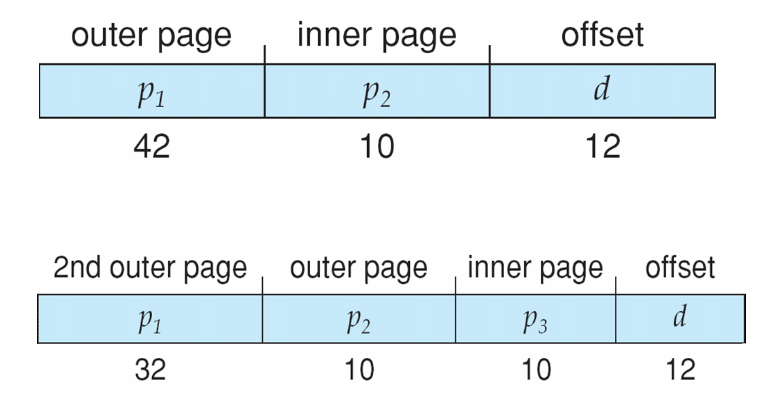
\includegraphics[scale=0.3]{24-tps.png}
\end{center}

\paragraph*{Hashed page tables} - comune in address spaces > 32 bits. Virtual page number hashed in page table (page tableul contine un lant de lemente hashate catre aceeasi locatie).
\subparagraph*{Fiecare element contine:} (1) virtual page number, (2) valoarea page frameului mapat, (3) un pointer la urmatorul element
\subparagraph*{Virtual page numbers:} comparate in aceasta cautare in lant pentru un match (daca e gasit, se extrage physical frameul)
\subparagraph*{CLustered page tables} e o variatie pentru 64-biti. La fel ca hashed, dar fiecare entry se refera la mai multe pagini (16). Foarte folositor pentru sparese address spaces (unde referintele la memorie nu sunt continue si sunt imprastiate)
\begin{center}
    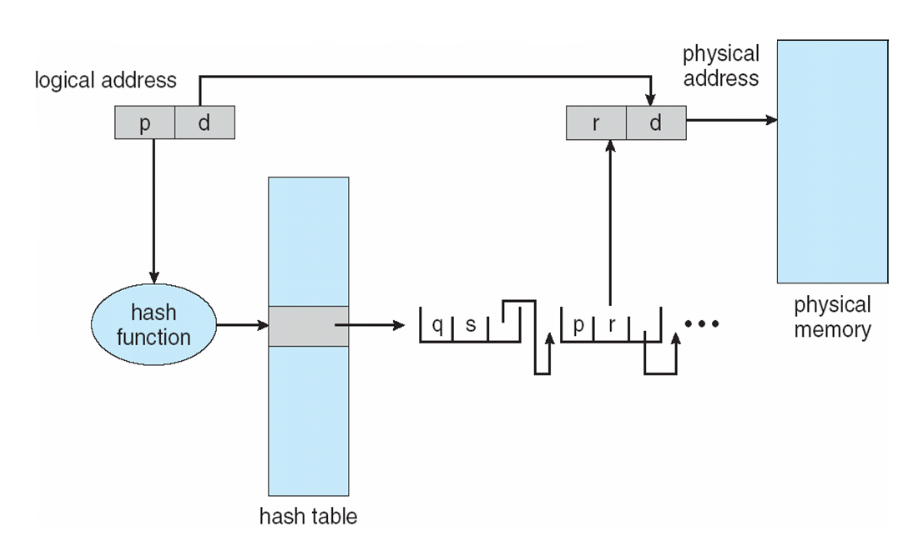
\includegraphics[scale=0.3]{25-hpt.png}
\end{center}

\paragraph*{Inverted Page Table}
\begin{enumerate}
    \item In loc ca fiecare proces sa aiba un page table si sa tina cont de toate logical pages posibile, trackuieste toate physical pages
    \item O intrare pentru fiecare pagina reala de memorie
    \item Intrarea consista in adresa virtuala a paginii stocate in acea locatie reala de memorie, cu informatia despre procesul care o detine
    \item Scade memoria pentru fiecare page table, dar creste timpul de cautare in tabel cand are o page reference
    \item Se poate folosi hashtable ca sa se limiteze cautarea la una sau cateva page-table enteries
\end{enumerate}
\begin{center}
    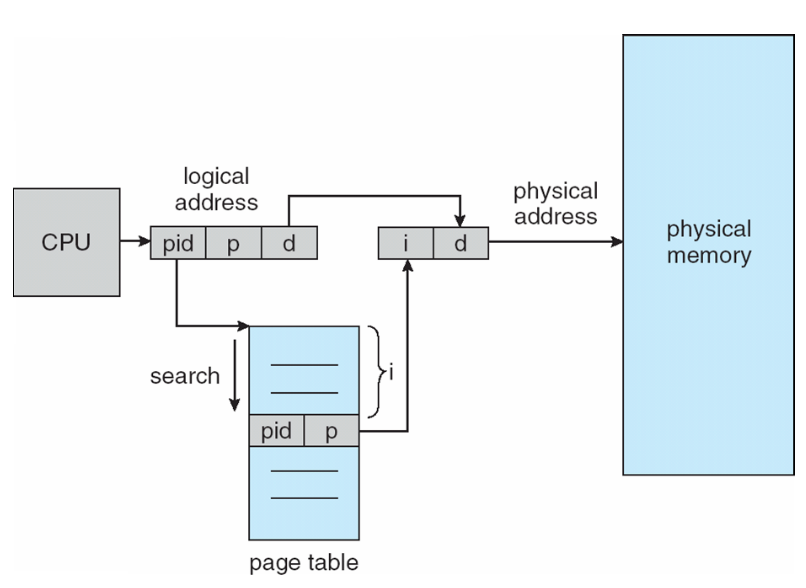
\includegraphics[scale=0.3]{26-ipt.png}
\end{center}

\subsection*{Swapping}
Un proces poate fi \textbf{swapped} temporar din memorie catre un backing store si apoi adus in memorie pentru continuarea executiei (memoria fizica total a proceselor poate sa depaseasca memoria fizica)
\paragraph*{Backing store} - disc rapid destul de mare cat sa acomodeze copii ale tuturor imaginiler din memorie pentru toti userii si sa dispuna de acces direct la aceste imagini de memorie
\paragraph*{Roll out, roll in} - un tip de swapping pentru priority-based scheduling unde procesele cu lower-priority sunt swappate ca sa faca loc proceselor higher-priority
\paragraph*{Transfer time} - cea mai mare parte din swap time
\paragraph*{Ready queue} - sistemul mentine aceasta coada cu procesele ready-to-run care au imagini de memorie pe disc

\paragraph*{Context switch time cu swapping} - daca urmatorul proces de pus pe cpu nu e in memorie, trebuie swapat cu altul, asa ca context switch time poate fi foarte mare. Sunt syscalluri de folosire a memoriei cu request\_memory() si release\_memory()
\subparagraph*{Restrictii:} I/O in asteptare nu poate fi swapat pentru ca ar fi in alt proces sau se poate transfera I/O catre kernel space apoi pe dispozitivul I/O (double buffering).
\subparagraph*{Strategia pe OS moderne:} swapeaza doar cand memoria libera e foarte mica

\subsection*{IA-32 Arch}
\begin{enumerate}
    \item Segementation si segmantation cu paging
    \item Fiecare segment e de 4GB, pana la 16K segmente per proces
    \item Divizata in 2 partitii
          \begin{enumerate}
              \item Prima partitie pana la 8K segmente sunt procesele private (\textbf{LDT} - local descriptor table)
              \item A doua paritie pana la 8K segmente partajate intre toate procesele (\textbf{GDT} - global descriptor table)
          \end{enumerate}
\end{enumerate}
\begin{center}
    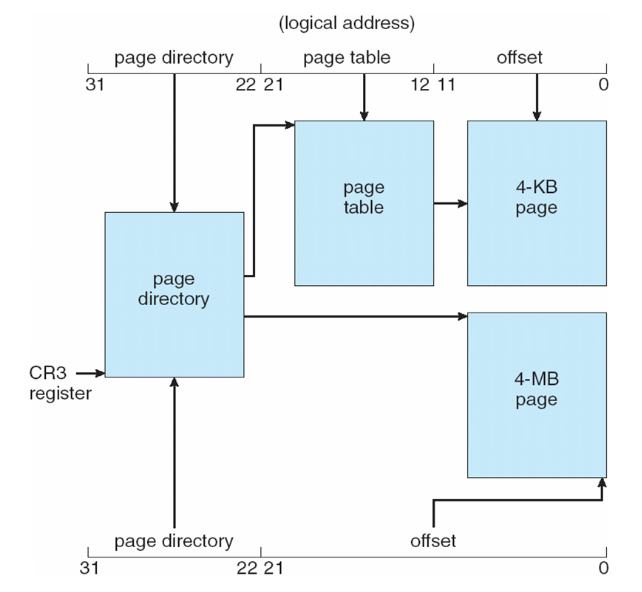
\includegraphics[scale=0.3]{27-32mem.png}
\end{center}

\subsection*{IA-32 cu PAE}
\begin{enumerate}
    \item Pagingul are o schema cu 3 nivele
    \item Primii 2 biti se refera la un \textbf{page directory pointer table}
    \item Page-directory si page-table au intrari de 64biti
    \item Efectul: cresterea spatiului de adresare la 36 biti - 64gb de memorie fizica
\end{enumerate}

\begin{center}
    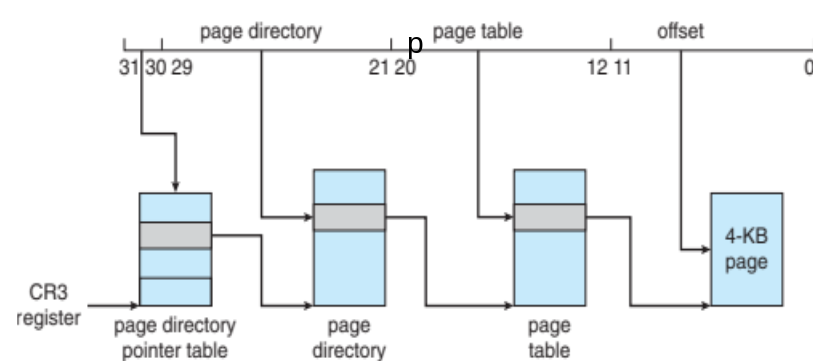
\includegraphics[scale=0.3]{28-32paemem.png}
\end{center}

\subsection*{Intel x86-64}
\paragraph*{48 bit addressing} - in practica asta este standardul implementat
\paragraph*{4 levels paging hierarchy}
\paragraph*{PAE} pentru 52 biti
\begin{center}
    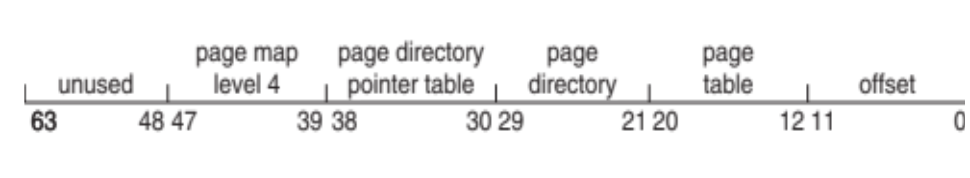
\includegraphics[scale=0.3]{29-64mem.png}
\end{center}


\section[Ch10 Virtual memory]{Virtual memory}
Separarea dintre memoria logica a utilizatorului de memoria fizica
\begin{enumerate}
    \item Doar o parte din program trebuie sa fie in memorie pentru executie
    \item Logical address space $\geq$ physical address space
    \item Address spaces shareuite intre procese
    \item Crearea de procese mai eficienta
    \item Mai multe programe pot rula in acelasi timp
    \item Mai putin I/O necesar pentru a face load sau swap pe procese
\end{enumerate}

\paragraph*{Implementare prin}
\begin{enumerate}
    \item Demand paging
    \item Demand segmentation
\end{enumerate}

\paragraph*{Virtual-address Space}
\begin{enumerate}
    \item De obicei spatiul de adresare logic pentru stack incepe la Max logical address si creste "in jos", in timp ce heapul creste "in sus" maximizand folosirea address space-ului, iar spatiul de adresare dintre ele este un hole (nu e nevoie de memorie fizica pana cand heapul sau stackul cresc peste o noua pagina)
    \item Foloseste sparese address spaces cu gauri lasate pentru crestere, dll-uri etc
    \item Librariile de sistem sunt shareuite prin mapping in virtual address space
    \item Memorie partajata prin maparea paginilor read-write in virtual address space
    \item Paginile pot fi shareuite in timpul unui fork() pentru a grabi crearea procesului
\end{enumerate}

\begin{center}
    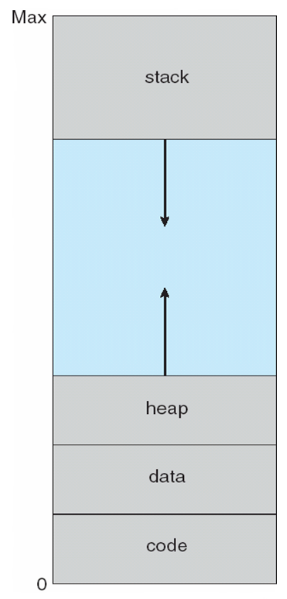
\includegraphics[scale=0.3]{30-vas.png}
\end{center}

\subsection*{Demand paging}
\begin{enumerate}
    \item Poate aduce intreg procesul in memorie la load sau doar o pagina cand este nevoie
    \item Similar cu paging cu swapping
    \item Daca o pagina e necesara $\rightarrow$ refer-o: referinta invalida $\rightarrow$ abort, not-in-memory $\rightarrow$ bring to memory
    \item \textbf{Lazy swapper} - nu swapeaza o pagina in memorie decat daca e necesara. Swapperul care se ocupa de pagini este \textbf{pager}
\end{enumerate}

\paragraph*{Concepte de baza} - Pagerul ghiceste ce pagini vor fi folosite pana sa le swapeze
\paragraph*{Valid-invalid bit} - cu fiecare intrare in page table se determina bitul valid-invalid asociat (v $\rightarrow$ in memorie, i $\rightarrow$ nu e in memorie). Daca MMU determina ca bitul este i, atunci da page fault
\begin{center}
    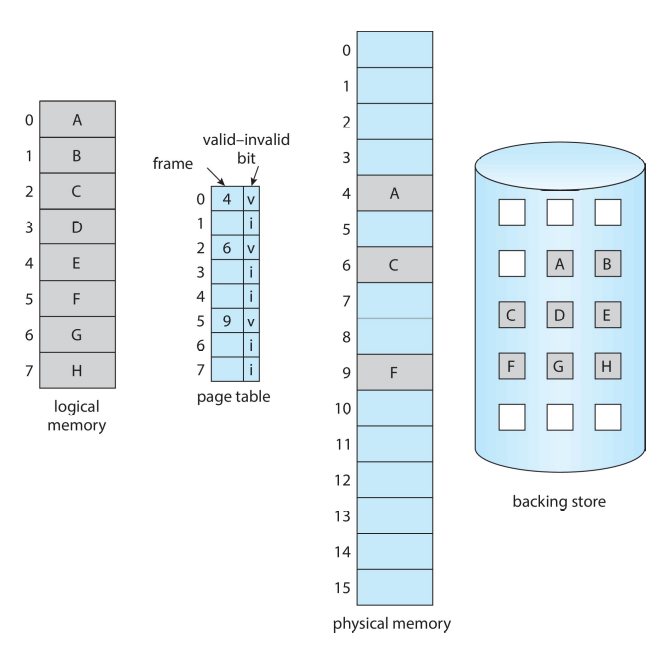
\includegraphics[scale=0.3]{31-vib.png}
\end{center}

\paragraph*{Pasi in rezolvarea page fault}
\begin{enumerate}
    \item Daa este o referinta la o pagina, prima referinta va fi trapata in OS: page fault
    \item OS se uita in alt tabel ca sa decida daca este referinta invalida (abort) sau doar nu este in memorie
    \item Gaseste un frame liber
    \item Swapeaza pagina in frame via scheduled disk operation
    \item Reseteaza tabelele sa indice ca pagina este acum in memorie si seteaza validation bit la v
    \item Reporneste instructiunea care a cauzat page fault
\end{enumerate}
\begin{center}
    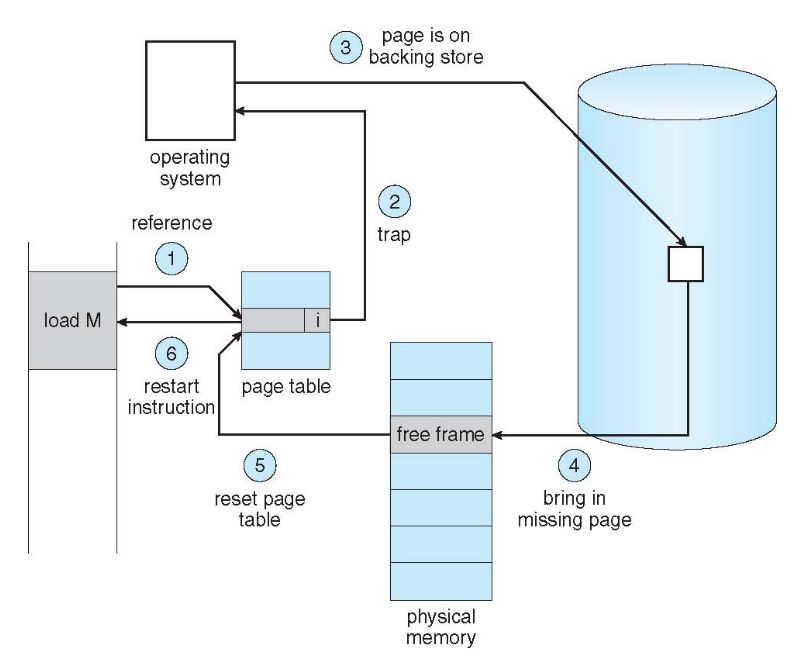
\includegraphics[scale=0.3]{32-pagefault.png}
\end{center}

\paragraph*{Aspecte ale demand paging}
\begin{enumerate}
    \item Caz extrem: porneste procesul fara pagini in memorie. OS seteaza IP catre prima instructiune a procesului si da page fault, apoi pentru celelalte pagini la primul acces (\textbf{pure demand paging})
    \item O instructiune poate referinta mai multe pagini. De exemplu fetch si decode a unei instructiuni care aduna 2 numere si stocheaza rezultatul in memorie. Se poate folosi pentru optimizare \textbf{locality of reference}
    \item Suport hardware necesar pentru demand paging
          \begin{enumerate}
              \item Page table cu bit valid/invalid
              \item Memorie secundara (device de swap cu swap space)
              \item Instructiunea restart
          \end{enumerate}
\end{enumerate}

\paragraph*{Free-frame list} - in caz de page fault, OS-ul trebuie sa aduca pagina dorita in memorie din secondary storage. Se implementeaza free-frame list - un pool de free frames pentru astfel de cerinte
\subparagraph*{Zero-fill-on-demand} - continutul frameurilor scos inainte de a fi alocat
\subparagraph*{Start up} - toata memoria disponibila e pusa pe un free-frame list

\paragraph*{Stadiile demand paging - cazul cel mai rau}
\begin{enumerate}
    \item Trap in OS
    \item Salveaza user registers si process state
    \item Determina daca interruptul a fost page fault
    \item Verifica daca acel page reference a fost legal pentru a determina locatia paginii pe disc
    \item Citeste de pe disc intr-un free frame
          \begin{enumerate}
              \item Asteapta in coada pentru dispozitiv pana cand toate requesturile de read au fost efectuate
              \item Asteapta dupa latenta dispozitivului si timpul de seek
              \item Incepe transferul paginii intr-un free frame
          \end{enumerate}
    \item Cat timp astepti, aloca CPU altui user
    \item Primeste un interrupt de la subsistemul disk I/O (completata)
    \item Salveaza registrii si process state pentru celelalt utilizator
    \item Determina daca interruptul a fost de la disk
    \item Corecteaza page table-ul cu alte tabele pentru a arata ca pagina este acum in memorie
    \item Asteapta ca CPU-ul sa fie alocat acestui proces din nou
    \item Restaureaza user registers, process state si noul page table, apoi rezuma instructiunea intrerupta
\end{enumerate}

\paragraph*{Performanta}: page fault rate $0 \leq p \leq 1$ (0 - fara, 1 - toate referintele sunt page faults)
\begin{center}
    \begin{math}
        EAT = (1-p) * memory\_access + p * (page\_fault\_overhead + swap\_page\_out + swap\_page\_in)
    \end{math}
\end{center}

\paragraph*{Optimizari}
\begin{enumerate}
    \item Viteza mai mare de swap space I/O fata de sistemul I/O chiar daca e pe acelasi dispozitiv (swap in bucati mai mari pentru ca e mai putin management necesar decat file system)
    \item Copiaza intreg procesul in swap space la load time, apoi page in si page out din swap space (versiuni mai vechi de BSD Unix)
    \item Cere page din binarul programului de pe disc, dar da discard decat paging out cand eliberezi un frame. Inca e nevoie de swap space: paginile neasociate cu un fisier (stack sau heap) sunt memorie anonima, paginile pot fi modificate in memorie, dar nu scrise imediat pe file system (Solaris si BSD-ul actual)
    \item Mobilele nu suporta swapping, dar cer pagina din file system si iau doar read-only pages (cum ar fi codul)
\end{enumerate}

\paragraph*{COW (copy-on-write)} - parintele si copiii shareuiesc initial aceleasi pagini in memorie (daca unul schimba o pagina, doar atunci e copiata).
\subparagraph*{}In general paginile libere sunt alocate dintr-un pool de zero-fill-on-demand pages
\subparagraph*{vfork()} e un syscall in care parintele suspenda folosirea de copil a COW in address space-ul parintelui (copilul poate executa exec() si e foarte eficient)
\paragraph*{Page replacement} (daca nu exista free frame)
\begin{enumerate}
    \item Previne supraalocarea memoriei prin modificarea rutinei de page-fault pentru a include page replacement
    \item Foloseste modify (dirty) bit pentru a reduce overheadul transfeurlui de pagini (doar paginile modificate sunt scrise pe disc)
    \item Completeaza separarea dintre memoria logica si cea fizica
\end{enumerate}
\subparagraph*{Algoritmul}
\begin{enumerate}
    \item Gaseste locatia paginii necesare pe disc
    \item Gaseste free frame (daca nu exista, foloseste replacement pentru a selecta victim frame si scrie victim frame pe disk daca e dirty)
    \item Adu pagina dorita intr-un nou free frame, actualizaeaza pagina si frame tables
    \item Continua procesul prin restartarea instructiunii care a cauzat trapul
\end{enumerate}
\subparagraph*{2 potentiale page transfers pentru page fault $\rightarrow$ EAT mai mare}
\begin{center}
    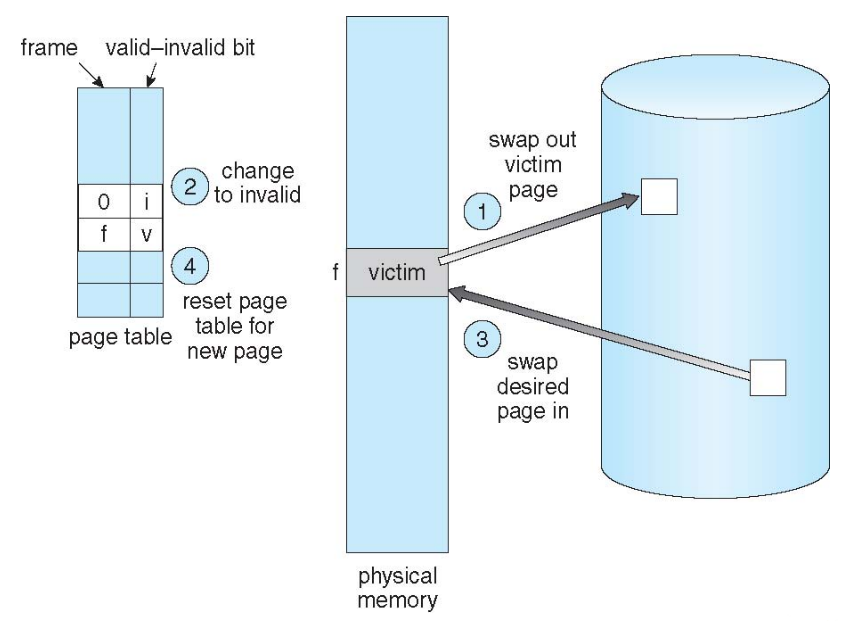
\includegraphics[scale=0.3]{33-pagereplacement.png}
\end{center}

\paragraph*{Algoritmii pentru page si frame replacement}
\subparagraph*{Frame-allocation} determina cate frameuri sa dea fiecarui proces si ce frameuri sa inlocuiasca
\subparagraph*{Page-replacement} Vrea page-fault rate minim atat la primul acces cat si la reaccesare

\paragraph*{FIFO}
\begin{enumerate}
    \item Stringul de referinte: 7,0,1,2,0,3,0,4,2,3,0,3,0,3,2,1,2,0,1,7,0,1
    \item 3 frameuri (3 pagini pot fi in memorie per proces)
\end{enumerate}

\subparagraph*{15 page faults}
\begin{center}
    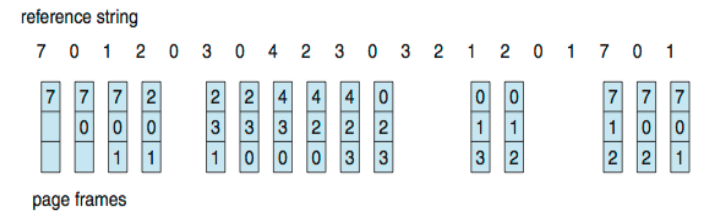
\includegraphics[scale=0.4]{34-fifopf.png}
\end{center}
\subparagraph*{Anomalia lui Belady} mai multe frameuri pot produce mai multe page faults

\paragraph*{Optimal Algorithm} Replace doar pe pagina care nu va fi folosita mai des in viitor
\begin{center}
    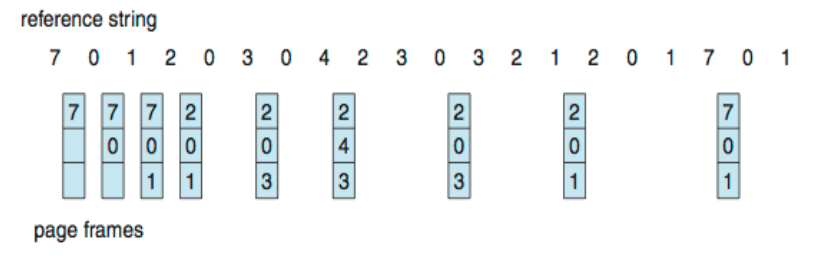
\includegraphics[scale=0.4]{35-optpf.png}
\end{center}

\paragraph*{LRU (least recently used)} - paginile cele mai vechi
\begin{center}
    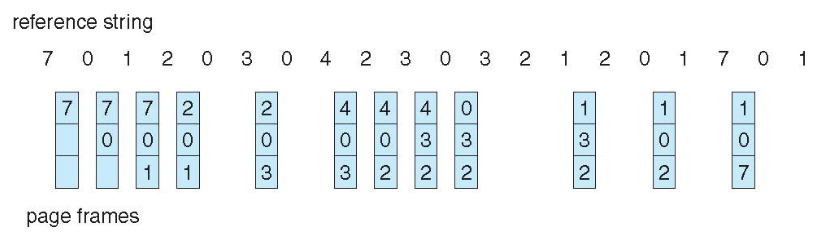
\includegraphics[scale=0.4]{36-lrupf.png}
\end{center}
\subparagraph*{12 faults} - mai bun ca FIFO, mai rau ca OPT
\subparagraph*{Implementare LRU}
\begin{enumerate}
    \item Counter
          \begin{enumerate}
              \item Fiecare pagina are un counter in care punem clock cand intra
              \item Cand trebuie schimbata o pagina, ne uitam la countere dupa valoarea cea mai mica (e nevoie de search table)
          \end{enumerate}
    \item Stack
          \begin{enumerate}
              \item Pastreaza o stiva cu double link
              \item Cand o pagina e referntiata: mut-o sus
              \item Fiecare update e mai scump, dar nu e nevoie de search pentru replacement
          \end{enumerate}
\end{enumerate}

\paragraph*{LRU si OPT} sunt cazuri de stack algorithms care nu au anomalia lui Belady

\paragraph*{LRU approximation algorithms} - e nevoie de hardware special si e tot incet
\subparagraph*{Reference bit} - fiecare pagina are un bit initial 0, cand e referntiata se face 1, apoi se face replacement pe orice pagina cu bit de referinta 0 (daca exista, daca nu, nu stim ordinea)
\subparagraph*{Second-chance algorithm} - in general FIFO plus reference bit pe hardware. Daca reference bit = 0 $\rightarrow$ replace, daca reference bit = 1 $\rightarrow$ seteaza-l ca 0 si las-o in memorie, treci la pagina urmatoare (aceleasi reguli)

\subparagraph*{Enhanced second-chance algorithm} - cu 2 biti: reference si modify
\begin{enumerate}
    \item Se ia perechea ordonata (reference, modify)
    \item (0,0) $\rightarrow$ nici folosita, nici modificata - cea mai buna
    \item (0,1) $\rightarrow$ nefolosita, dar modificata - trebuie write out inainte de replacement
    \item (1,0) $\rightarrow$ folosita recent, dar curata - probabil va fi folosita curand
    \item (1,1) $\rightarrow$ Recent folosita si modificata - probabil va fi folosita curand si trebuie write out pana la replacement
\end{enumerate}

\paragraph*{Counting algorithms} - se pastreaza un counter cu numarul de referinte care au fost facute catre o pagina (nu e comun). \textbf{LFU} (least frequently used) - replacement pe pagina cu counterul cel mai mic, \textbf{MFU} - replacement cu counterul cel mai mare (se considera ca cea cu counterul cel mai mic doar a fost adusa si trebuie folosita)

\paragraph*{Page-buffering algorithms}
\begin{enumerate}
    \item Tine un pool de free frames
          \begin{enumerate}
              \item Cand un frame e necesar, e valabil
              \item Citeste pagina intr-un free frame si selecteaza victima evacuarii si adaugarii in free pool
              \item Cand e convenient, evacueaza victima
          \end{enumerate}
    \item Tine o lista de pagini modificate (posibil) - cand backing store este idle, scrie paginile acolo si seteaza-le ca non-dirty
    \item TIne o lista de continut intact de free frames si noteaza ce e in el - daca e referntiata pana sa fie refolosita, nu e enevoie sa iei continutul din nou de pe disc, folosit in special pentru a reduce penalizarea daca victima gresita a fost selectata
\end{enumerate}

\subsection*{Allocation of frames}
2 scheme majore de alocare (cu mai multe variante)
\begin{enumerate}
    \item Fixed allocation
    \item Priority allocation
\end{enumerate}

\paragraph*{Fixed Allocation}
\begin{enumerate}
    \item Fixa: 100 frameuri, 5 procese, da 20 frameuri per proces (se pot tine unele libere in buffer pool)
    \item Proportionala: in functie de marimea procesului (poate fi dinamic, pentru ca procesele isi pot schimba marimea)
\end{enumerate}
\subparagraph*{Exemplu}
\begin{enumerate}
    \item $s_i$ = marimea procesului $p_i$
    \item $S = \sum s_i$
    \item m = numarul total de frameuri
    \item $a_i$ = alocarea pentru $p_i$, $a_i = \frac{s_i}{S}*m$
\end{enumerate}
\begin{center}
    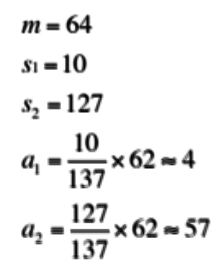
\includegraphics[scale=0.4]{37-fixedalloc.png}
\end{center}

\paragraph*{Global vs. Local Allocation}
\subparagraph*{Global replacement} - procesul selecteaza un replacement frame din multimea tuturor (poate lua frameul altuia) - execution time per proces poate varia semnificativ, dar are throughput mai mare deci e mai comun
\subparagraph*{Local replacement} - fiecare proces selecteaza din multimea frameurilor alocate - mai consistent in performanta per-proces, dar posibil sa subutilizeze memoria

\subsection*{Reclaiming pages}
\begin{enumerate}
    \item Strategie de a implementa global page-replacement policy
    \item Toate cererile din memorie sunt satisfacute din free-frame list, nu se asteapta ca lista sa ajunga la 0 pana incepem sa selectam pagini pentru replacement
    \item Replacement trigger cand lista e mai mica de un prag
    \item Strategia incearca sa faca posibil spatiu suficient de memorie pentru noi cereri in orice moment
\end{enumerate}

\subsection*{NUMA}
Viteza de acces la memorie variaza. Performanta optima cand se aloca memorie "aproape" de CPU-ul in care threadul e scheduled. Solaris a introdus \textbf{lgroups} - structura care trackuieste CPU/Memory low latency groups si cand e posibil, pune toate threadurile unui proces si aloca toata memoria acelui proces intr-un lgroup
\begin{center}
    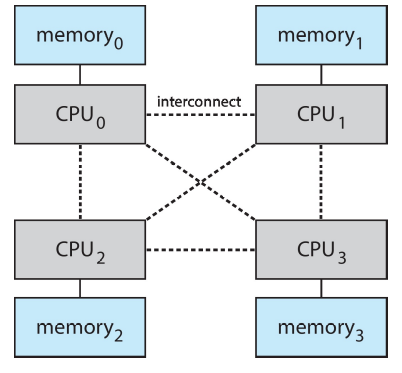
\includegraphics[scale=0.4]{38-numa.png}
\end{center}

\subsection*{Thrashing}
Daca un proces nu are "suficiente" pagini, page-fault e foarte mare
\begin{enumerate}
    \item Page fault ca sa ia pagina
    \item Replacement pe frameul existent
    \item E nevoie de replacement frame inapoi rapid
    \item Duce la
          \begin{enumerate}
              \item CPU utilizat putin
              \item OS crede ca trebuie sa creasca gradul de multiprogramming
              \item Inca un proces este adaugat in sistem
          \end{enumerate}
\end{enumerate}

\paragraph*{Locality} - o multime de pagini folosite impreuna. Modelul localitatii spune ca atunci cand un proces se executa, se muta dintr-o localitate in alta (unele pot sa se suprapuna). De exemplu, cand o functia este apelata, se defineste o noua localitate, iar cand iese, atunci si procesul iese din acea localitate

\subparagraph*{Working-Set Model} - daca alocam suficiente frameuri pentru a acomoda localitatea curenta, va da page fault doar cand se muta intr-o alta, dar daca alocam mai putine decat localitatea curenta, procesul are sanse sa faca thrashing.
\subparagraph*{D} - total demand pentru frameuri si WSS este working setul pentru procesul i. $D=\sum WSS_i$
\begin{enumerate}
    \item $D>m$ (total demand > numarul de frameuri), atunci va fi trashing pentru ca un proces nu poate avea suficiente frameuri
    \item $D\leq m$, nu va fi trashing
\end{enumerate}

\subparagraph*{Page-fault frequency} - abordare mai directa decat WSS. Se stabileste o rata acceptabila de PFF si o politica de replacement locala. Daca rata e joasa, procesele pierd frame, daca e prea mare, primesc frame

\subsection*{Allocating Kernel Memory}
Tratata diferit de user memory si alocata de obice intr-un pool de free-memory.

\paragraph*{Buddy System} - aloca memorie dintr-un segment cu marime fixa consistand in pagini fizice continue. Se aloca folosind \textbf{power-of-2 allocator}.
\subparagraph*{Avantaj} - coalesce rapid din bucatile nefolosite intr-o bucata mai mare
\subparagraph*{Dezavantaj} - fragmentare

\paragraph*{Slab Allocator} - strategie alternanta
\subparagraph*{Slab} e una sau mai multe pagini fizice continue
\subparagraph*{Cache} contine mai multe slaburi
\begin{enumerate}
    \item Un cache pentru o structura de date unica a kernelului
    \item Fiecare cache e umplut cu obiecte
    \item Cand e creat e marcat cu obiecte free
    \item Cand sunt stocate structurile de date, obiectele sunt marcate ca used
    \item Daca slabul e full cu obiecte, urmatorul obiect e alocat unui slab vid (daca nu e niciunul vid, se aloca altul)
    \item Avantaj: fara fragmentare si stasiface accesul rapid la memorie
\end{enumerate}

\subparagraph*{Dupa Linux 2.2} avem SLOB (simple list of blocks - tine 3 obiecte pentru obiecte mici, medii si mari) si SLUB (salb optimizat pentru performanta, pentru ca nu are cozi per-CPU, iar metadata e stocata in structura paginii)

\begin{center}
    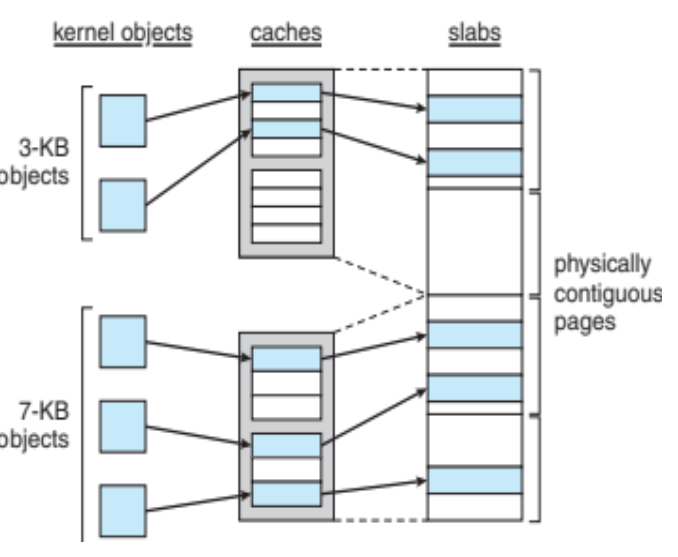
\includegraphics[scale=0.4]{39-slab.png}
\end{center}

\subsection*{Prepaging}
Pentru a reduce numarul mare de page faults care se intampla la startupul unui porces. Daca sunt nefolosite, I/O si memoria au fost risipite.
\paragraph*{Presupunem} s pagini prepaged si $\alpha$ procentul de pagini folosite. Atunci $s*\alpha$ este costul de a salva page faults si $s*(1-\alpha)$ numarul de pagini nenecesare. Asadar, cand $\alpha$ e aproape de zero $\rightarrow$ apar pierderi din prepaging

\subsection*{Page Size}
\paragraph*{Consideratii necesare}
\begin{enumerate}
    \item fragmentare
    \item page table size
    \item resolution
    \item I/O overhead
    \item numarul de page faults
    \item localitatea
    \item marimea TLB si eficienta sa
    \item Mereu puteri ale lui 2
    \item In medie, cresc in timp
\end{enumerate}

\subsection*{TLB Reach}
Cantitatea de memorie accesibila din TLB
\begin{center}
    \begin{math}
        TLB\ Reach = (TLB\ Size) * (Page\ Size)
    \end{math}
\end{center}
\begin{enumerate}
    \item De obicei intreg wss-ul unui proces e stocat in TLB, atlfel are multe page faults
    \item Creste page size poate duce la cresterea fragmentarii
    \item Mai multe page sizes face posibil ca aplicatiile sa ceara page sizes mai mari fara sa creasca fragmentarea
\end{enumerate}

\subsection*{Program structure}
\begin{center}
    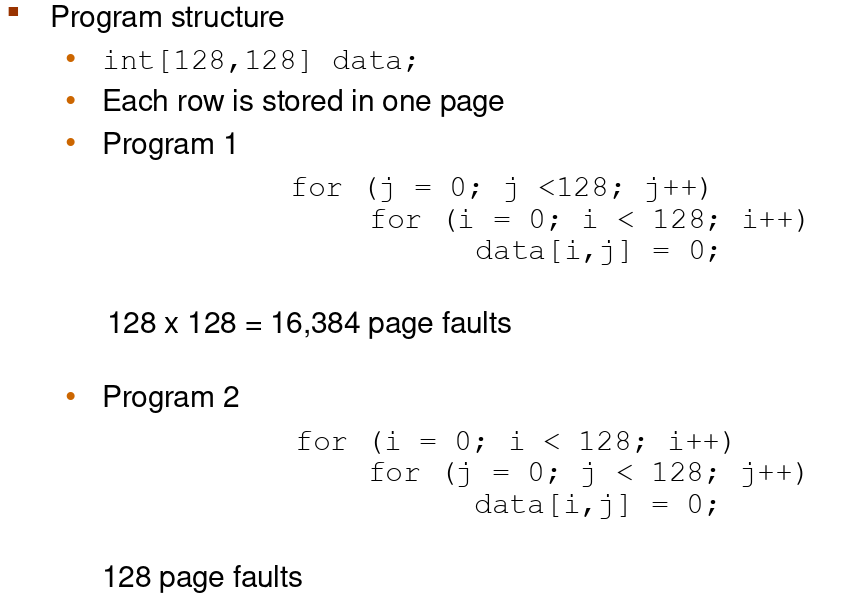
\includegraphics[scale=0.4]{40-progstruct.png}
\end{center}

\subsection*{I/O Interlock}
Uneori paginile trebuie sa fie blocate in memorie. De exemplu la copierea fisierelor dintr-un dispozitiv, paginile trebuie sa fie blocakte (locked) de a fi evacuate de replacement. Se poate face pinning paginilor ce trebuie sa fie blocate in memorie.

\subsection*{Operatori}
\begin{enumerate}
    \item REG - 0 frames
    \item ADD MOV SUB - 1 frame
    \item MUL DIV - 2 frames
    \item (doar) [\dots] - 1 frame
          \begin{enumerate}
              \item ADD REG REG - 1 frame
              \item MUL REG REG - 2 frames
              \item ADD REG [\dots] - 2 frames
              \item ADD [\dots] [\dots] - 3 frames
              \item MUL REG [\dots] - 3 frames
              \item MUL [\dots] [\dots] - 4 frames
          \end{enumerate}
\end{enumerate}

\section[Ch13 File system interface]{File system interface}
Spatiul logic de adresare continuu.
\subsection*{Tipuri}
\begin{enumerate}
    \item Data
          \begin{enumerate}
              \item Numeric
              \item Character
              \item Binary
          \end{enumerate}
    \item Program
\end{enumerate}

\subsection*{Atribute}
\begin{enumerate}
    \item Nume
    \item Identifier
    \item Type
    \item Location
    \item Size
    \item Protection
    \item Time, date, user identification
    \item Poate include atribute extinse: checksum
\end{enumerate}

\subsection*{Directory Structure}
Colectie de noduri care contin informatii despre toate fisierele. Atat structura de directoare cat si fisierele rezida pe disc

\subsection*{Operatii}
\begin{enumerate}
    \item Create
    \item Write (scrie la locatia pointerului)
    \item Read (citeste la locatia pointerului)
    \item Reposition within a file (seek)
    \item Delete
    \item Truncate
    \item Open($F_i$) - cauta in directory structure intrarea $F_i$ si muta-i continutul in memorie
    \item Close($F_i$) - muta continutul intrarii $F_i$ din memorie in structura de directoare de pe disc
\end{enumerate}

\subsection*{Open Files}
\paragraph*{Open-file table} - tracking pe fisierele deschise
\paragraph*{File pointer} - pointer la ultima locatie de read/write, per proces care are fisierul deschis
\paragraph*{File-open count} - counter pe numarul de deschidere a fisierului (pentru a permite stergerea datelor din open-file table cand ultimul proces o inchide)
\paragraph*{DIsk location} - cache de informatii de acces ale datelor
\paragraph*{Access rights} - modul de acces al informatiei per proces

\subsection*{File Locking}
Folosit de unele OS si FS. Similar cu reader-writer locks.
\paragraph*{Shared lock} - ca un reader-lock: mai multe procese pot folosi concurent
\paragraph*{Exclusive lock} - ca un writer lock
\paragraph*{Mediaza accesul la un fisier}
\begin{enumerate}
    \item Mandatory - accesul este respins in functie de lock-urile tinute si cele cerute
    \item Advisory - procesul poate vedea statusul lockurilor si decide ce sa faca
\end{enumerate}

\subsection*{Logical records}
Un fisier e logical records de marime fixa

\subsection*{Sequential access}
\begin{enumerate}
    \item Read next
    \item Write next
    \item Reset
    \item no read after last write (rewrite)
\end{enumerate}

\subsection*{Direct Access}
\begin{enumerate}
    \item read n
    \item write n
    \item position to n
          \begin{enumerate}
              \item read next
              \item write next
              \item rewrite n
          \end{enumerate}
\end{enumerate}

Numerele de block relative permit OS sa decida unde sa puna fisierul.

\subsection*{Alte metode de acces}
De obicei au un \textbf{index} pentru fisier pe care il tin in memorie ca sa determine rapid unde sunt datele pe care sa opereze. Daca indexul e prea mare, se creaza un in-memory index care-l indexeaza pe cel de pe disc

\subsection*{Disk structure}
\paragraph*{Partitii} - discul poate fi subdivizat in partitii
\paragraph*{RAID} - discul sau partitiile pot fi protejate de failure
\paragraph*{Folosirea} raw sau formatata cu un FS
\paragraph*{Sinonime pentru partitii:} minidisks, slices
\paragraph*{Volume} - entitatea care contine FS
\paragraph*{Tracking pe FS} - volumul trackuieste informatiile FS-ului in device directory sau volume table of contents
\paragraph*{Special-purpose file systems} - folosite impreuna cu general-purpose file systems

\subsection*{Program structure}
\begin{center}
    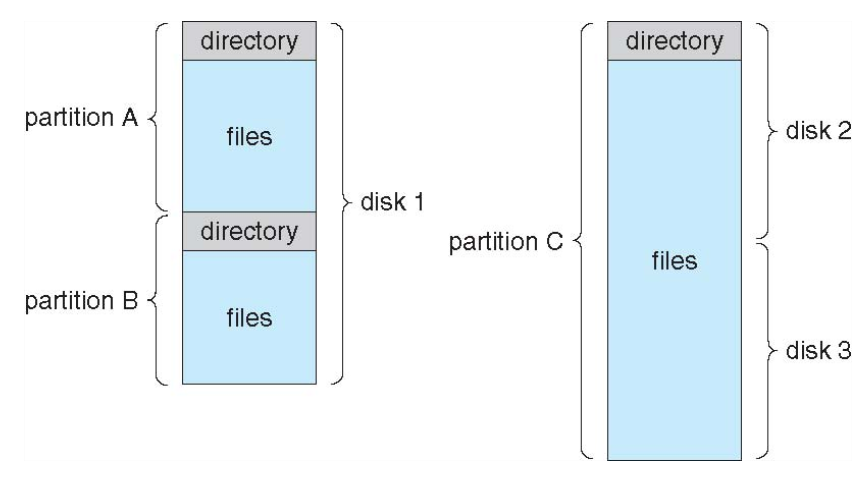
\includegraphics[scale=0.4]{41-fsorg.png}
\end{center}

\subsection*{Types of File Systems}
\paragraph*{Solaris}
\begin{enumerate}
    \item tmpfs - memory based FS volatil pentru I/O rapid si temporar
    \item objfs - interfata la memoria kernelului pentru a lua kernel symbols pentru debugging
    \item ctfs - contract file system pentru daemoni
    \item lofs - loopback fs care permite ca un FS sa fie accesat in locul altuia
    \item procfs - interfata a kernelului catre structura de procese
    \item ufs, zfs - general purpose file systems
\end{enumerate}

\subsection*{Operatii pe director}
\begin{enumerate}
    \item Search file
    \item create file
    \item delete file
    \item list a directory
    \item rename a file
    \item traverse the FS
\end{enumerate}

\subsection*{Directory Organization}
\paragraph*{Pentru a obtine}
\begin{enumerate}
    \item Eficienta (localizarea rapida a unui fisier)
    \item Denumire
          \begin{enumerate}
              \item 2 utilizatori pot avea acelasi nume pentru fisiere diferite
              \item Acelasi fisier poate avea mai multe nume
          \end{enumerate}
    \item Grupare
\end{enumerate}

\subsection*{Single-level directory}
Acelasi director pentru toti userii
\begin{center}
    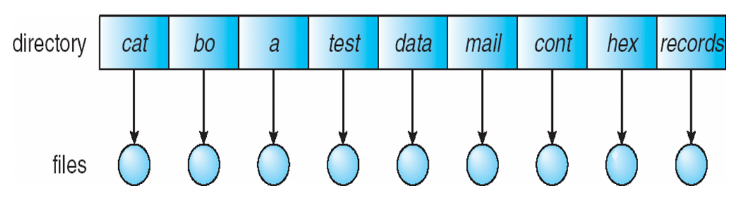
\includegraphics[scale=0.4]{42-sld.png}
\end{center}

\subsection*{2-level directory}
Fiecare user cu director separat
\begin{enumerate}
    \item Poate avea fisiere cu nume identice pentru utilizatori diferiti
    \item Searching eficient
    \item Nu se pot grupa
\end{enumerate}
\begin{center}
    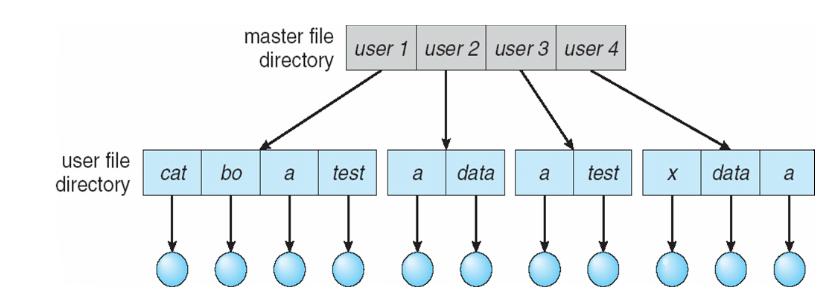
\includegraphics[scale=0.4]{43-tld.png}
\end{center}

\subsection*{Tree-structured Directories}
\begin{center}
    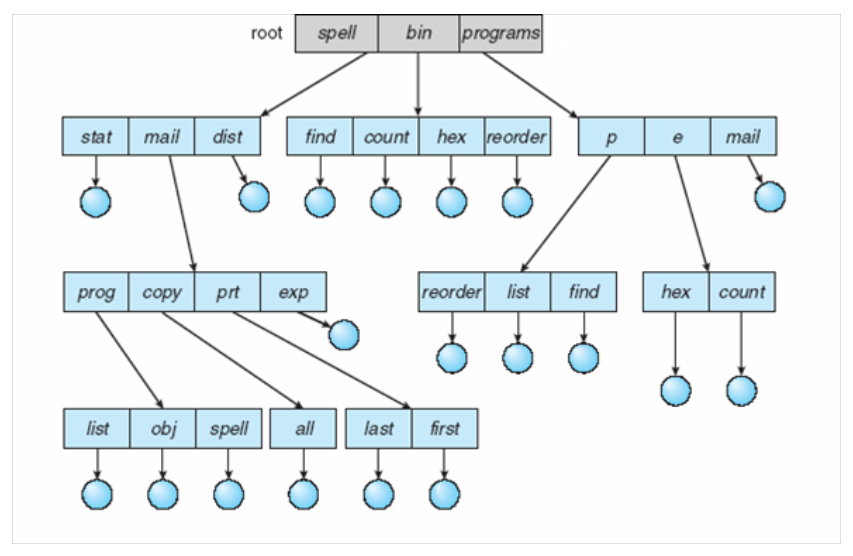
\includegraphics[scale=0.4]{44-tsd.png}
\end{center}

\subsection*{Acyclic-Graph Directories}
Au subdirectoare si fisiere shared
\begin{center}
    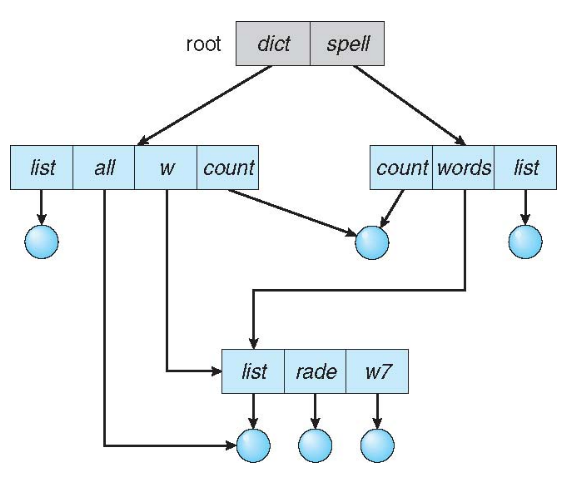
\includegraphics[scale=0.4]{45-agd.png}
\end{center}

\begin{enumerate}
    \item Aliasing (2 nume diferite)
    \item Daca dict sterge w/list $rightarrow$ dangling pointer
          \begin{enumerate}
              \item Se pot pune backpointeri ca sa stergem toti pointerii
              \item Backpointeri cu daisy chain organization
              \item Entry-hold-count
          \end{enumerate}
    \item Tip de director nou
          \begin{enumerate}
              \item link - un alt nume catre un fisier existent
              \item resolve the link - urmareste pointerul pentru a localiza fisierul
          \end{enumerate}
\end{enumerate}

\subsection*{General Graph Directory}
\begin{center}
    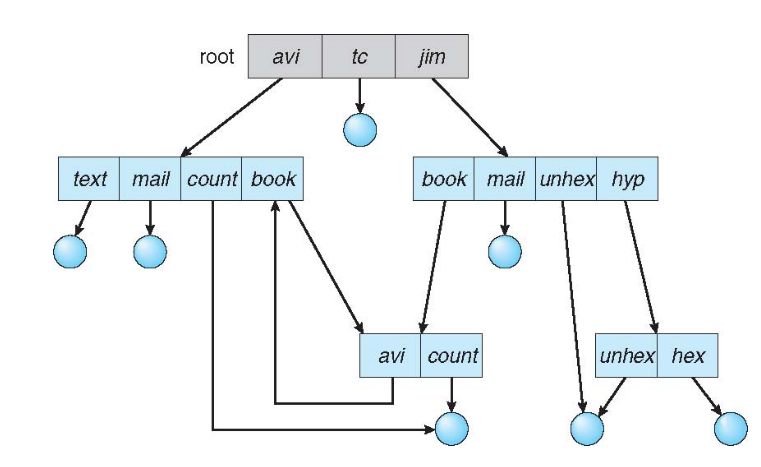
\includegraphics[scale=0.4]{46-ggd.png}
\end{center}
\paragraph*{Problema ciclurilor:} link catre fisiere, nu subdirectoare; garbage collection; la fiecare link foloseste un algoritm de detectie a ciclurilor pentru a vedea daca este ok

\subsection*{File protection}
Ownerul trebuie s controleze ce poate fi facut si de cine poate fi facut
\paragraph*{Tipuri de acces}
\begin{enumerate}
    \item read
    \item write
    \item execute
    \item append
    \item delete
    \item list
\end{enumerate}


\section[Ch14 File system implementation]{File system implementation}
\subsection*{FS Structure}
\begin{enumerate}
    \item Rezida pe secondary storage (disks)
    \item e o interfata a utilizatorului catre sotrage, mapand logical catre physical
    \item acces eficient si convenient la disc, permitand ca datele sa fie stocate, locate si scoase usor
    \item Discul pune la dispozitie in-place rewrite si random access (de obicei transferurile sunt in blocuri de sectoare - de obicei 512bytes)
    \item \textbf{FCB} (file control block) - structura de stocare care consista in informatii despre un fisier
    \item Device driverul controleaza dipsozitivul fizic
    \item FS organizat in layere
\end{enumerate}

\begin{center}
    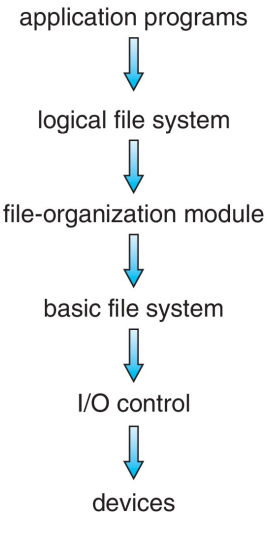
\includegraphics[scale=0.4]{47-layeredfs.png}
\end{center}

\subsection*{FS Layers}
\paragraph*{Device drivers} gestioneaza dispozitivele I/O la layerul de control I/O
\paragraph*{Basic file system} - primeste o comanda si o traduce driverului
\paragraph*{Gestioneaza} buffere si cacheuri (bufferele tin datele in tranzit, cacheurile tin datele cele mai des folosite)
\paragraph*{File organization module} - intelege fisierele, adresele logice si blocurile fizice. Traduce blocuri logice in blocuri fizice. Gestioneaza spatiul liber si alocarea pe disc
\paragraph*{Logical file system} - gestioneaza metadatele. Traduce numele fisierului in file number, file handle si locatie prin gestionarea file control blocks (inodes in UNIX). Face managementul directoarelor si protectia.
\paragraph*{Avantaj} - reduce complexitatea si redundanta
\paragraph*{Dezavantaj} - are overhead
\paragraph*{Layerele logice} pot fi implementate de catre designerul de OS

\subsection*{FS Operations}
\paragraph*{Boot control block} - contine informatiile necesare sistemului sa booteze OS din acel volum (necesar daca contine OS, de obicei e primul block al volumului)
\paragraph*{Volume control block} - superblock, master file table - contine detaliile volumului
\paragraph*{DIrectory structure} - nume si numere inode, MFT (master file table)

\subsection*{FCB (File Control Block)}
\paragraph*{OS-ul} mentine FCB per fisier

\subsection*{In-Memory FS Structures}
\paragraph*{Mount table} tine toate system mounts, mount points si FS types
\paragraph*{System-wide open-file table} o copie a FCB pentru fiecare fisier si alte informatii
\paragraph*{Per-process open-file table} contine pointer la intrari din system-wide open-file table, dar si alte informatii

\subsection*{Directory implementation}
\paragraph*{Linear list} de nume de fisiere cu pointeri catre blocurile de date.
\begin{enumerate}
    \item Simplu de programat
    \item Costisitor ca executie (timp de cautare liniar, pot fi ordonate alfabetic cu o lista inlantuita sau cu un B+ tree)
\end{enumerate}

\paragraph*{Hash table} - lista liniara cu strucura datelor hashed
\begin{enumerate}
    \item Timp mai mic de cautare
    \item Coliziuni - daca 2 nume de fisiere au acelasi hash catre aceeasi locatie
    \item BUn doar daca intrarile sunt fixe sau se foloseste chained-overflow method
\end{enumerate}

\subsection*{Allocation Method}
\paragraph*{Alocare continua} - fiecare fisier ocupa o multime continua de blocuri
\begin{enumerate}
    \item Simplu - trebui doar locatia de start si lungimea
    \item Probleme
          \begin{enumerate}
              \item Gasirea spatiului pe disc pentru un fisier
              \item Sa stii marimea exacta a unui fisier
              \item Fragmentare externa (e nevoie de compaction off-line care presupune downtime sau on-line)
          \end{enumerate}
\end{enumerate}

\paragraph*{Extent-based systems} - aloca blocuri de disc in extents. Extent e un bloc continuu de disc. Un fisier poate avea unul sau mai multe extenturi. Ex: Veritas File System

\paragraph*{Linked allocation} - fiecare fisier e linkuita unei liste de blocuri si se termina la pointerul nul
\begin{enumerate}
    \item Nu exista fragmentare externa
    \item Fiecare bloc contine pointer catre urmatorul
    \item Fara compaction, external fragmentation
    \item Cand e nevoie de un bloc, se cheama free space management system
    \item Se poate imbunatati eficienta prin blocks clustering in grupuri, dar creste fragmentarea interna
    \item Unreliable
    \item Cautarea unui bloc poate sa ia multe seekuri de I/O
\end{enumerate}
\begin{center}
    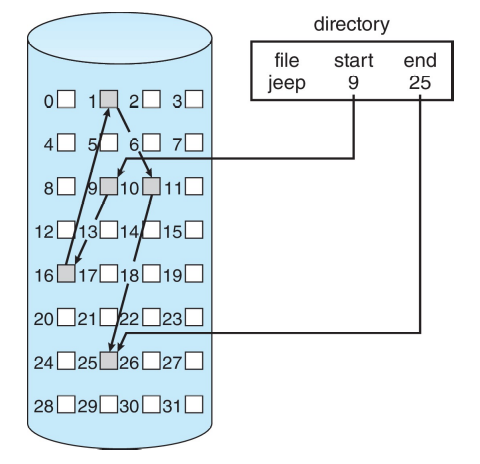
\includegraphics[scale=0.4]{48-linkedalloc.png}
\end{center}

\paragraph*{FAT} - inceputul volumului are un tabel indexat dupa block number. E ca o linked list, dar mai rapid si cacheable. Alocarea unui bloc nou e simpla.

\paragraph*{Indexed Allocation Method} - fiecare fisier are propriul bloc de indecsi cu pointeri catre propriile data blocks
\subparagraph*{Fisiere mici}
\begin{enumerate}
    \item E nevoie de un index table
    \item Acces random
    \item Acces dinamic fara fragmentare externa, dar are overhedului blocului de indecsi
    \item Maparea din logic in fizic intr-un fisier de maximum 256KB si un bloc de 512bytes necesita doar 1 bloc pe tabel de indecsi
\end{enumerate}
\subparagraph*{Fisiere mari} - maparea se face cu linked scheme (link blocks of index table) si multi-level indexing

\subsection*{Free space management}
\paragraph*{Bit vector/bit map} de n blocuri
\paragraph*{Se calculeaza} numarul de bits pe word * numarul de 0-valued words + offsetul primului bit
\begin{center}
    \includegraphics[scale=0.4]{49-linkedfreespacelist.png}
\end{center}

\paragraph*{Grouping} - se modifica linked list sa stocheze adresa urmatoarelor n-1 blocuri libere in primul bloc liber, plus un pointer catre primul bloc care contine free-block-pointers
\paragraph*{Continuing} - pentru ca spatiul este frecvent folosit in mod continuu si eliberat cu alocare continua, extents sau clustering: se tine adresa primului bloc liber si numarul de blocuri care il urmeaza, iar lista spatiului liber are intrari care contin adrese si counts

\paragraph*{Space maps}
\begin{enumerate}
    \item FOlosite in ZFS
    \item considera metadatele I/O pe FS foarte mari - structuri mari ca bit maps nu pot intra in memorie ceea ce duce la multe I/O
    \item divide spatiul in unitati metslabs si gestioneaza metslabs
    \item fiecare metsalb e asociat cu un space map
    \item tine evidenta in log file, nu in FS
    \item activitatea metaslab e mapata ca un balanced-tree in memorie, indexata dupa offset (se poate da replay la log, se pot comnbina blocuri libere continue intr-o singura intrare)
\end{enumerate}

\paragraph*{TRIMing unused blocks}
HDD-urile pot face overwrite in place. NVM-urile sufera pentru ca trebuie sa stearga inainte de a scrie, iar stergerile sunt incete. TRIM e un mecanism care infomreaza NV-urile ca acea pagina e libera pentru garbage collection sau daca blocul e liber, acum poate fi sters.

\subsection*{Eficienta si performanta}
\paragraph*{Eficienta}
\begin{enumerate}
    \item Alocarea pe disc si algoritmii de directoare
    \item Tipuirle de date tinute in intrare de fisiere din director
    \item Pre-alocarea sau alocarea as-needed metadatelor structurilor
    \item Structuri cu marime fixa sau variabila
\end{enumerate}

\paragraph*{Performanta}
\begin{enumerate}
    \item Tinerea datelor si metadatelor impreuna
    \item Buffer cache - sectiune separata in main memory pentru blocurile folosite des
    \item Scrieri sincrone unoeri cerute de programe sau de OS (cele asincrone sunt mai comune, bufferabile si rapide)
    \item Free-behind si read-ahead pentru a optimiza accesul secvential
    \item Readuri mai incete ca writeuri
\end{enumerate}

\paragraph*{Page cache} - cacheuieste pagini in loc de disk blocks cu tehnici de memorie virtuala si adrese. I/O mapate in memorie folosesc page cache
\begin{center}
    \includegraphics[scale=0.4]{50-pagecache.png}
\end{center}

\paragraph*{Unified buffer cache} - foloseste acelasi page cache ca sa cacheuiasca atat paginile mapate in memorie cat si fisiere normale de system I/O pentru a evita double caching
\begin{center}
    \includegraphics[scale=0.4]{51-ubc.png}
\end{center}

\subsection*{Recovery}
\paragraph*{Consistency checking} - comapra data din directory structure cu data blocks pe disc si fixeaza incosistentele.
\paragraph*{Backup} pe un alt dispozitiv
\paragraph*{Restoring} a datelor din backup

\subsection*{Log structured FS}
\paragraph*{Log structured/journaling} tin un sistem actualizat de metadate in file system ca transactii
\begin{enumerate}
    \item Tranzactiile sunt logate - sunt considerate committed in momentul in care apar in log (secvential)
    \item Tranzactiile din log sunt scrise asincron in structurile FS (cand structurile sunt modificate, sunt scoase din log)
    \item Daca FS crashuieste, toate tranzactiile ramase in log trebuie facute
    \item Recovery rapid de la crash cu sanse mici de inconsistente ale datelor
\end{enumerate}

\end{document}